\documentclass[12pt,]{article}
\usepackage{lmodern}
\usepackage{amssymb,amsmath}
\usepackage{ifxetex,ifluatex}
\usepackage{fixltx2e} % provides \textsubscript
\ifnum 0\ifxetex 1\fi\ifluatex 1\fi=0 % if pdftex
  \usepackage[T1]{fontenc}
  \usepackage[utf8]{inputenc}
\else % if luatex or xelatex
  \ifxetex
    \usepackage{mathspec}
  \else
    \usepackage{fontspec}
  \fi
  \defaultfontfeatures{Ligatures=TeX,Scale=MatchLowercase}
\fi
% use upquote if available, for straight quotes in verbatim environments
\IfFileExists{upquote.sty}{\usepackage{upquote}}{}
% use microtype if available
\IfFileExists{microtype.sty}{%
\usepackage{microtype}
\UseMicrotypeSet[protrusion]{basicmath} % disable protrusion for tt fonts
}{}
\usepackage[margin=1.0in]{geometry}
\usepackage{hyperref}
\hypersetup{unicode=true,
            pdftitle={Seasonal Dynamics of Epiphytic Microbial Communities on Marine Macrophyte Surfaces},
            pdfborder={0 0 0},
            breaklinks=true}
\urlstyle{same}  % don't use monospace font for urls
\usepackage{graphicx,grffile}
\makeatletter
\def\maxwidth{\ifdim\Gin@nat@width>\linewidth\linewidth\else\Gin@nat@width\fi}
\def\maxheight{\ifdim\Gin@nat@height>\textheight\textheight\else\Gin@nat@height\fi}
\makeatother
% Scale images if necessary, so that they will not overflow the page
% margins by default, and it is still possible to overwrite the defaults
% using explicit options in \includegraphics[width, height, ...]{}
\setkeys{Gin}{width=\maxwidth,height=\maxheight,keepaspectratio}
\IfFileExists{parskip.sty}{%
\usepackage{parskip}
}{% else
\setlength{\parindent}{0pt}
\setlength{\parskip}{6pt plus 2pt minus 1pt}
}
\setlength{\emergencystretch}{3em}  % prevent overfull lines
\providecommand{\tightlist}{%
  \setlength{\itemsep}{0pt}\setlength{\parskip}{0pt}}
\setcounter{secnumdepth}{0}
% Redefines (sub)paragraphs to behave more like sections
\ifx\paragraph\undefined\else
\let\oldparagraph\paragraph
\renewcommand{\paragraph}[1]{\oldparagraph{#1}\mbox{}}
\fi
\ifx\subparagraph\undefined\else
\let\oldsubparagraph\subparagraph
\renewcommand{\subparagraph}[1]{\oldsubparagraph{#1}\mbox{}}
\fi

%%% Use protect on footnotes to avoid problems with footnotes in titles
\let\rmarkdownfootnote\footnote%
\def\footnote{\protect\rmarkdownfootnote}

%%% Change title format to be more compact
\usepackage{titling}

% Create subtitle command for use in maketitle
\providecommand{\subtitle}[1]{
  \posttitle{
    \begin{center}\large#1\end{center}
    }
}

\setlength{\droptitle}{-2em}

  \title{\textbf{Seasonal Dynamics of Epiphytic Microbial Communities on Marine
Macrophyte Surfaces}}
    \pretitle{\vspace{\droptitle}\centering\huge}
  \posttitle{\par}
    \author{}
    \preauthor{}\postauthor{}
    \date{}
    \predate{}\postdate{}
  
\usepackage{times} % Times New Roman font
\usepackage[T1]{fontenc}

\usepackage[none]{hyphenat}

\usepackage{setspace}
\doublespacing
\setlength{\parskip}{1em}

\usepackage{lineno}
\renewcommand{\linenumberfont}{\normalfont\tiny}

\usepackage{pdfpages}

\usepackage{indentfirst}

\usepackage[labelsep=period, labelfont=bf]{caption}
\renewcommand{\thefigure}{\arabic{figure}}
\renewcommand{\figurename}{Fig.}
\captionsetup{justification=raggedright,singlelinecheck=false}

\usepackage{pdflscape}
\newcommand{\blandscape}{\begin{landscape}}
\newcommand{\elandscape}{\end{landscape}}

\usepackage{siunitx}
\DeclareSIUnit\molar{\mole\per\cubic\deci\metre}
\DeclareSIUnit\Molar{\textsc{m}}
\DeclareSIUnit\cells{\text{cells}}

\usepackage{caption}
\captionsetup{justification=justified}

\usepackage{float}

\usepackage{xr}
\externaldocument[supp-]{supplementary}

\usepackage{txfonts}

\renewcommand{\figureautorefname}{Fig.}

\usepackage{microtype}

\begin{document}
\maketitle

\vspace{20mm}

Marino Korlević\textsuperscript{1\(*\)}, Marsej
Markovski\textsuperscript{1}, Zihao Zhao\textsuperscript{2}, Gerhard J.
Herndl\textsuperscript{2,3}, Mirjana Najdek\textsuperscript{1}

1. Center for Marine Research, Ruđer Bošković Institute, Croatia

2. Department of Functional and Evolutionary Ecology, University of
Vienna, Austria

3. NIOZ, Department of Marine Microbiology and Biogeochemistry, Royal
Netherlands Institute for Sea Research, Utrecht University, The
Netherlands

\textsuperscript{\(*\)}To whom correspondence should be addressed:

Marino Korlević

G. Paliaga 5, 52210 Rovinj, Croatia

Tel.: +385 52 804 768

Fax: +385 52 804 780

e-mail:
\href{mailto:marino.korlevic@irb.hr}{\nolinkurl{marino.korlevic@irb.hr}}

Running title: Seasonal dynamics of epiphytic communities

\newpage
\linenumbers
\sisetup{mode=text}
\setlength\parindent{24pt}

\hypertarget{summary}{%
\subsection{Summary}\label{summary}}

Surfaces of marine macrophytes (seagrasses and macroalgae) are inhabited
by diverse microbial communities. Most studies focusing on epiphytic
communities of macrophytes did not take into account temporal changes or
applied low sampling frequency approaches. Illumina sequencing of the V4
16S rRNA region was performed to determine the seasonal dynamics of
epiphytic communities of the seagrass \emph{Cymodocea nodosa} and
invasive macroalga \emph{Caulerpa cylindracea}. Leaves and thalli were
sampled in a meadow of \emph{Cymodocea nodosa} invaded by the invasive
\emph{Caulerpa cylindracea} and in a monospecific settlement of
\emph{Caulerpa cylindracea} located in the proximity of the meadow at
monthly intervals. For comparison the ambient prokaryotic plankton
community was also characterized. At the OTU level, the microbial
community composition differed between the ambient water and the
epiphytic communities exhibiting host-specificity. Also, successional
changes were observed connected to the macrophyte growth cycle.
Taxonomic analysis, however, showed similar high rank groups in the
ambient water and the epiphytic communities, with the exception of
\emph{Desulfobacterota}, which were only found on \emph{Caulerpa
cylindracea}. \emph{Cyanobacteria} showed seasonal changes while other
high rank taxa were present throughout the year. Phylogenetic groups
present throughout the year constituted most of the sequences, while
less abundant taxa showed seasonal patterns connected to the macrophyte
growth cycle. Taken together, epiphytic microbial communities of the
seagrass \emph{Cymodocea nodosa} and the macroalgae \emph{Caulerpa
cylindracea} appear to be host-specific and contain taxa that undergo
successional changes.

\newpage

\hypertarget{introduction}{%
\subsection{Introduction}\label{introduction}}

Marine macrophytes (seagrasses and macroalgae) are important ecosystem
engineers forming close associations with microorganism belonging to all
three domains of life (Egan \emph{et al.}, 2013; Tarquinio \emph{et
al.}, 2019). Microbes can live within macrophyte tissue as endophytes or
can form epiphytic communities on surfaces of leaves and thalli (Egan
\emph{et al.}, 2013; Hollants \emph{et al.}, 2013; Tarquinio \emph{et
al.}, 2019). Epiphytic and endophytic microbial communities exhibit a
close functional relationship with the macrophyte host. It was proposed
that this close relationship constitutes a holobiont, an integrated
community where the macrophyte organism and its symbiotic partners
support each other (Margulis, 1991; Egan \emph{et al.}, 2013; Tarquinio
\emph{et al.}, 2019).

Biofilms of microbial epiphytes can contain diverse taxonomic groups and
harbor cell abundances from 10\textsuperscript{2} to
10\textsuperscript{7} \si{\cells\per\cm\squared} (Armstrong \emph{et
al.}, 2000; Bengtsson \emph{et al.}, 2010; Burke and Thomas \emph{et
al.}, 2011). In such an environment a number of positive and negative
interactions between the macrophyte and the colonizing microorganisms
have been described (Egan \emph{et al.}, 2013; Hollants \emph{et al.},
2013; Tarquinio \emph{et al.}, 2019). Macrophytes can promote growth of
associated microbes by nutrient exudation, while in return
microorganisms may support macrophyte performance through improved
nutrient availability, phytohormone production and protection from toxic
compounds, oxidative stress, biofouling organisms and pathogens (Egan
\emph{et al.}, 2013; Hollants \emph{et al.}, 2013; Tarquinio \emph{et
al.}, 2019). Besides these positive interactions, macrophytes can
negatively impact the associated microbes such as pathogenic bacteria by
producing reactive oxygen species and secondary metabolites (Egan
\emph{et al.}, 2013; Hollants \emph{et al.}, 2013; Tarquinio \emph{et
al.}, 2019).

All these ecological roles are carried out by a taxonomically diverse
community of microorganisms. At higher taxonomic ranks a core set of
macrophyte epiphytic taxa was described consisting mainly of
\emph{Alphaproteobacteria}, \emph{Gammaproteobacteria},
\emph{Desulfobacterota}, \emph{Bacteroidota}, \emph{Cyanobacteria},
\emph{Actinobacteriota}, \emph{Firmicutes}, \emph{Planctomycetota},
\emph{Chloroflexi} and \emph{Verrucomicrobiota} (Crump and Koch, 2008;
Tujula \emph{et al.}, 2010; Lachnit \emph{et al.}, 2011). In contrast,
at lower taxonomic ranks host specific microbial communities were found
(Lachnit \emph{et al.}, 2011; Roth-Schulze \emph{et al.}, 2016).
Recently, it was shown that even different morphological niches within
the same alga had a higher influence on the composition of the bacterial
community than biogeography or environmental factors (Morrissey \emph{et
al.}, 2019). While the microbial community composition varies between
host species, metagenomic analyses revealed that the majority of the
microbial functions are conserved (Burke and Peter Steinberg \emph{et
al.}, 2011; Roth-Schulze \emph{et al.}, 2016). This discrepancy between
the microbial taxonomic and functional composition might be explained by
the lottery hypothesis. It postulates that an initial random
colonization step takes places from a set of functionally equivalent
taxonomic groups resulting in taxonomically different epiphytic
communities sharing a core set of functional genes (Burke and Peter
Steinberg \emph{et al.}, 2011; Roth-Schulze \emph{et al.}, 2016). In
addition, some of the variation in the reported data could be attributed
to different techniques used in these studies, such as different
protocols for epiphytic cell detachment and/or DNA isolation, as no
standard protocol has been yet established to study epiphytic
communities (Ugarelli \emph{et al.}, 2019; Korlević \emph{et al.},
submitted).

The majority of studies describing macrophyte epiphytic microbial
communities did not include possible seasonal changes (Crump and Koch,
2008; Lachnit \emph{et al.}, 2009; Burke and Thomas \emph{et al.}, 2011;
Roth-Schulze \emph{et al.}, 2016; Ugarelli \emph{et al.}, 2019). If
seasonal changes were taken into account, low temporal frequency,
applied methodologies and/or limited number of analyzed host species did
not allow a high taxonomic resolution (Tujula \emph{et al.}, 2010;
Lachnit \emph{et al.}, 2011; Miranda \emph{et al.}, 2013; Michelou
\emph{et al.}, 2013; Mancuso \emph{et al.}, 2016). In the present study
we describe the seasonal dynamics of bacterial and archaeal communities
on the surfaces of the seagrass \emph{Cymodocea nodosa} and siphonous
macroalgae \emph{Caulerpa cylindracea} determined on a mostly monthly
scale. Bacterial and archaeal epiphytes were sampled in a meadow of
\emph{C. nodosa} invaded by the invasive \emph{C. cylindracea} and in a
locality of only \emph{C. cylindracea} located in the proximity of the
seagrass meadow. For comparison, the microbial community of the ambient
seawater was also characterized.

\newpage

\hypertarget{results}{%
\subsection{Results}\label{results}}

Sequencing of the 16S rRNA V4 region yielded a total of 1.8 million
sequences after quality curation and exclusion of sequences without
known relatives (no relative sequences) and eukaryotic, chloroplast and
mitochondrial sequences (\autoref{supp-nseq_notus}). A total of 35
samples originating from epiphytic archaeal and bacterial communities
associated with surfaces of the seagrass \emph{C. nodosa} and the
macroalga \emph{C. cylindracea} were analyzed. In addition, 18 samples
(one of the samples was sequenced twice) originating from the ambient
seawater were also processed for comparison. The number of reads per
sample ranged between 8,408 and 77,463 sequences
(\autoref{supp-nseq_notus}). Even when the highest sequencing effort was
applied the rarefaction curves did not level off as commonly observed in
high-throughput 16S rRNA amplicon sequencing approaches
(\autoref{supp-rarefaction}). Following quality curation and exclusion
of sequences as mentioned above reads were clustered into 28,750
different OTUs at a similarity level of 97 \si{\percent}. Read numbers
were normalized to the minimum number of sequences (8,408,
\autoref{supp-nseq_notus}) through rarefaction resulting in 17,145
different OTUs with 365 to 2,036 OTUs per sample
(\autoref{supp-calculators}). To determine seasonal changes in richness
and diversity the observed number of OTUs, Chao1, ACE, Exponential
Shannon (Jost, 2006) and Inverse Simpson were calculated after
normalization through rarefaction. Generally, richness estimators and
diversity indices showed similar trends. On average, higher values were
found for \emph{C. cylindracea} (mixed {[}Number of OTUs, 1,680.3 ±
125.3 OTUs{]} and monospecific {[}Number of OTUs, 1,737.9 ± 164.5
OTUs{]}) than for \emph{C. nodosa} (Number of OTUs, 1,059.6 ± 211.0
OTUs) and lowest values were obtained for the microbial community of the
ambient seawater (Number of OTUs, 523.4 ± 136.0 OTUs)
(\autoref{supp-calculators}). Seasonal changes did not reveal such large
dissimilarities. \emph{C. nodosa} communities showed a slow increase
towards the end of the study, while \emph{C. cylindracea} (mixed and
monospecific) communities were characterized by slightly higher values
in spring and summer than in autumn and winter
(\autoref{supp-calculators}).

To determine the proportion of shared archaeal and bacterial OTUs and
communities sampled in different environments the Jaccard's Similarity
Coefficient on presence-absence data and Bray-Curtis Similarity
Coefficient, respectively, were calculated. Coefficients were determined
after normalization through rarefaction and binning of samples from the
particular environment. The highest proportion of shared OTUs and
community was found between mixed and monospecific \emph{C. cylindracea}
(Jaccard, 0.35; Bray-Curtis, 0.77), while lower shared values were
calculated between ambient seawater and epiphytic communities
(\autoref{matrix}). Shared proportion between \emph{C. nodosa} and
\emph{C. cylindracea} were approximately in-between the values of mixed
and monospecific \emph{C. cylindracea}. To assess seasonal changes in
the proportion of shared OTUs and communities the Jaccard's and
Bray-Curtis Similarity Coefficients were calculated between consecutive
sampling points (\autoref{shared}). Both coefficients showed similar
trends. Temporal proportional changes were more pronounced for ambient
seawater than for \emph{C. nodosa} and especially \emph{C. cylindracea}
associated communities (\autoref{shared}). In addition, only 0.4 -- 1.0
\si{\percent} of OTUs from each surface associated community were
present at all seasons. These persistent OTUs constituted a high
proportion of total sequences (40.4 -- 53.9 \si{\percent}). To further
disentangle the environmental and seasonal community dissimilarity a
Principal Coordinates Analysis (PCoA) based on Bray-Curtis distances and
OTU abundances was applied. A clear separation between ambient seawater
and surface associated communities was found (\autoref{pcoa}). In
addition, a separation of epiphytic bacterial and archaeal communities
based on host species was detected. This separation was further
supported by ANOSIM (R = 0.96, \emph{p} \textless{} 0.001). Seasonal
changes of \emph{C. nodosa} associated communities indicated a
separation between spring, summer and autumn/winter samples (ANOSIM, R =
0.53, \emph{p} \textless{} 0.01). For \emph{C. cylindracea} associated
communities a separation between summer and autumn/winter/spring samples
was observed that was, however, not as strong as for \emph{C. nodosa}
associated communities (ANOSIM, R = 0.31, \emph{p} \textless{} 0.01)
(\autoref{pcoa}).

The taxonomic composition of both, macrophyte associated and ambient
seawater communities was dominated by bacterial (99.1 ± 2.1
\si{\percent}) over archaeal sequences (0.9 ± 2.1 \si{\percent})
(\autoref{community}). Higher relative abundances of chloroplast related
sequences were only observed in surface associated communities, with
higher values in autumn/winter (37.2 ± 11.2 \si{\percent}) than in
spring/summer (20.9 ± 9.7 \si{\percent}) (\autoref{supp-chloroplast}).
Generally, at higher taxonomic ranks (phylum-class), epiphytic and
ambient seawater microbial communities were composed of similar
bacterial taxa. Ambient seawater communities were mainly comprised of
\emph{Actinobacteriota}, \emph{Bacteroidota}, \emph{Cyanobacteria},
\emph{Alphaproteobacteria}, \emph{Gammaproteobacteria} and
\emph{Verrucomicrobiota}. Communities associated with \emph{C. nodosa}
consisted additionally of \emph{Planctomycetota} contributing more in
summer 2018 than in other seasons. In addition, communities from mixed
and monospecific \emph{C. cylindracea} were similar and characterized by
the same groups as ambient seawater and \emph{C. nodosa} communities
with the addition of \emph{Desulfobacterota} (\autoref{community}).
Larger differences between environments and host species were observed
at lower taxonomic ranks (Figs. \ref{cyano} -- \ref{desulfo}).

\emph{Cyanobacteria} related sequences comprised, on average, 5.5 ± 4.4
\si{\percent} of total sequences (\autoref{cyano}). Higher proportions
were found for \emph{C. nodosa} (16.4 ± 5.3 \si{\percent}) and \emph{C.
cylindracea} mixed (7.7 ± 3.9 \si{\percent}) and monospecific (7.8 ± 2.4
\si{\percent}) associated communities in autumn and for ambient seawater
communities in winter (8.8 ± 7.5 \si{\percent}). Large taxonomic
differences between surface associated and ambient seawater
cyanobacterial communities were observed. Ambient seawater communities
were mainly comprised of \emph{Cyanobium} and \emph{Synechococcus},
while surface associated communities were comprised of
\emph{Pleurocapsa} and sequences within the class \emph{Cyanobacteriia}
that could not be further classified (no relative \emph{Cyanobacteriia})
(\autoref{cyano}). In addition, seasonal changes in surface associated
communities were observed in \emph{Pleurocapsa} and no relative
\emph{Cyanobacteriia} comprising larger proportions in autumn and winter
and \emph{Acrophormium}, \emph{Phormidesmis} and sequences without known
relatives within the \emph{Nodosilineaceae} (no relative
\emph{Nodosilineaceae}) in spring and summer (\autoref{cyano}).

Sequences classified as \emph{Bacteroidota} comprised, on average, 19.2
± 5.5 \si{\percent} of all sequences (\autoref{bactero}). Similarly to
\emph{Cyanobacteria}, large differences in the taxonomic composition
between ambient seawater and surface associated communities were found
(\autoref{bactero}). The ambient seawater community was characterized by
the NS4 and NS5 marine groups, uncultured \emph{Cryomorphaceae},
uncultured \emph{Flavobacteriaceae}, NS11-12 marine group,
\emph{Balneola}, uncultured \emph{Balneolaceae} and \emph{Formosa}. In
contrast, in surface associated communities \emph{Lewinella},
\emph{Portibacter}, \emph{Rubidimonas}, sequences without known
relatives within the \emph{Saprospiraceae} (no relative
\emph{Saprospiraceae}), uncultured \emph{Saprospiraceae}, (sequences
without known relatives within the \emph{Flavobacteriaceae} (no relative
\emph{Flavobacteriaceae})and uncultured \emph{Rhodothermaceae} were
found. Some groups showed minor seasonal changes such as no relative
\emph{Flavobacteriaceae} whose sequences were more abundant from
November 2017 until June 2018. In contrast, uncultured
\emph{Rhodothermaceae} showed higher proportions from June 2018 until
the end of the study period. Surface associated \emph{Bacteroidota}
communities were very diverse as observed in the high proportion of taxa
clustering as other \emph{Bacteroidota} (\autoref{bactero}).

On average, \emph{Alphaproteobacteria} were in comparison to the other
high rank taxa the largest taxonomic group, comprising 29.2 ± 12.0
\si{\percent} of all sequences (\autoref{alpha}). In accordance to the
above described taxa, large differences between ambient seawater and
surface associated communities were observed. Ambient seawater
communities were composed mainly of the SAR11 clade, AEGEAN-169 marine
group, SAR116 clade, sequences without known relatives within the
\emph{Rhodobacteraceae} (no relative \emph{Rhodobacteraceae}), HIMB11
and the OCS116 clade, while surface associated communities were composed
mainly of no relative \emph{Rhodobacteraceae} and to a lesser degree of
\emph{Pseudoahrensia}, \emph{Amylibacter} and sequences without known
relatives within the \emph{Alphaproteobacteria} (no relative
\emph{Alphaproteobacteria}) and \emph{Hyphomonadaceae} (no relative
\emph{Hyphomonadaceae}). Representatives of no relative
\emph{Rhodobacteraceae} comprised on average 40.6 ± 23.2 \si{\percent}
of all alphaproteobacterial sequences in the epiphytic community
(\autoref{alpha}). In addition, \emph{Amylibacter} was detected mainly
in \emph{C. nodosa} from November 2017 until March 2018.

Sequences related to \emph{Gammaproteobacteria} comprised on average
18.6 ± 3.9 \si{\percent} of all sequences (\autoref{gamma}). Similar to
above mentioned taxa, large taxonomic differences between ambient
seawater and surface associated communities were found. Ambient seawater
communities were mainly comprised of the OM60 (NOR5) clade,
\emph{Litoricola}, \emph{Acinetobacter} and the SAR86 clade, while
epiphytic communities were mainly composed of sequences without known
relatives within the \emph{Gammaproteobacteria} (no relative
\emph{Gammaproteobacteria}) and \emph{Granulosicoccus}. Beside these two
groups specific to all three epiphytic communities, \emph{C. nodosa} was
characterized by \emph{Arenicella}, \emph{Methylotenera} and sequences
without known relatives within the \emph{Burkholderiales} (no relative
\emph{Burkholderiales}), while \emph{Thioploca}, \emph{Reinekea} and
sequences without known relatives within \emph{Cellvibrionaceae} (no
relative \emph{Cellvibrionaceae}) were more specific to both mixed and
monospecific \emph{C. cylindracea}. In addition, \emph{Arenicella} was
more pronounced in November and December 2017, while no relative
\emph{Burkholderiales} and \emph{Methylotenera} were characteristic for
the period from March until May 2018. For the \emph{C. cylindracea}
specific taxa no relative \emph{Cellvibrionaceae} and \emph{Reinekea}
showed seasonality and were characteristic for samples originating from
June to October 2018. In addition, similar to \emph{Bacteroidota}, a
large proportion of the surface associated community was grouped as
other \emph{Gammaproteobacteria} indicating high diversity within this
group (\autoref{gamma}).

\emph{Desulfobacterota} were specific for \emph{C. cylindracea}. In the
mixed and monospecific \emph{C. cylindracea} communities the proportion
of \emph{Desulfobacterota} was 25.7 ± 11.2 \si{\percent} and 24.0 ± 4.3
\si{\percent}, respectively (\autoref{desulfo}). In contrast, in ambient
seawater and \emph{C. nodosa} communities the contribution of
\emph{Desulfobacterota} was only 0.1 ± 0.08 \si{\percent} and 1.0 ± 0.7
\si{\percent}, respectively. In \emph{C. cylindracea} the community
consisted mainly of \emph{Desulfatitalea}, \emph{Desulfobulbus},
\emph{Desulfopila}, \emph{Desulforhopalus}, \emph{Desulfotalea},
SEEP-SRB4, uncultured \emph{Desulfocapsaceae} and sequences without
known relatives within the \emph{Desulfobacteraceae} (no relative
\emph{Desulfobacteraceae}), \emph{Desulfobulbaceae} (no relative
\emph{Desulfobulbaceae}) and \emph{Desulfocapsaceae} (no relative
\emph{Desulfocapsaceae}) (\autoref{desulfo}).

\newpage

\hypertarget{discussion}{%
\subsection{Discussion}\label{discussion}}

Surfaces of marine macrophytes harbor biofilms consisting of diverse
microbial taxa (Egan \emph{et al.}, 2013; Tarquinio \emph{et al.},
2019). No standard protocol has been developed to study these
macophyte-associated microbes (Ugarelli \emph{et al.}, 2019). Different
procedures for removal of microbial cells from host surfaces are
described, such as host tissue shaking (Nõges \emph{et al.}, 2010),
scraping (Uku \emph{et al.}, 2007), swabbing (Mancuso \emph{et al.},
2016) and ultrasonication (Cai \emph{et al.}, 2014). All these methods
result in different removal efficiencies but none was enabling a
complete removal of attached microbial cells based on our experience. In
the present study, we applied a removal protocol (Korlević \emph{et
al.}, submitted) based on direct cellular lysis (Burke \emph{et al.},
2009). The application of a direct lysis procedure coupled with a high
sampling frequency and Illumina amplicon sequencing has enabled us to
described in detail the bacterial and archaeal communities associated
with the surfaces of two marine macrophytes, \emph{C. nodosa} and
\emph{C. cylindracea}.

In the present study, highest richness was observed for \emph{C.
cylindracea} (mixed and monospecific) followed by \emph{C. nodosa} and
lowest richness was found in ambient seawater microbial communities.
Higher richness of microbial communities associated with seagrasses than
in ambient seawater was described earlier and could be attributed to a
larger set of inhabitable microniches existing on macrophyte surfaces
than in the ambient seawater (Ugarelli \emph{et al.}, 2019). The highest
richness observed for \emph{C. cylindracea} might be partly due to its
contact with the sediment. The stolon of \emph{C. cylindracea} is
attached to the sediment surface with rhizoids and thus, the stolon and
rhizoids are in a direct contact with the sediment. In addition,
seasonal differences in richness observed for surface attached
communities indicated a slightly higher richness in spring and summer.
This pattern could be explained by a higher macrophyte growth in these
two seasons than in autumn and winter (M. Najdek, personal
communication; Zavodnik \emph{et al.}, 1998; Ruitton \emph{et al.},
2005). During their main growth season in spring and summer macrophytes
exhibit a more dynamic chemical interaction with the surface community
probably causing an increase in the number of inhabitable microniches
(Borges and Champenois, 2015; Rickert \emph{et al.}, 2016).

We observed a strong differentiation between the surface attached and
ambient seawater communities at the level of OTUs, in agreement with
most published studies (Burke and Thomas \emph{et al.}, 2011; Michelou
\emph{et al.}, 2013; Roth-Schulze \emph{et al.}, 2016; Mancuso \emph{et
al.}, 2016; Crump \emph{et al.}, 2018; Ugarelli \emph{et al.}, 2019).
This indicates that marine macrophytes are a selecting factor from the
pool of microbial taxa present in the ambient seawater, modifying the
microbial community once the macrophyte associated microbial biofilm
develops (Salaün \emph{et al.}, 2012; Michelou \emph{et al.}, 2013). In
contrast, Fahimipour \emph{et al.} (2017) report in a global study of
\emph{Zostera marina}, similarities between the microbial community
developed on leaves and in the ambient seawater. The discrepancy between
our data and the study of Fahimipour \emph{et al.} (2017) could be
explained by different seagrass species, methodological variations or
biogeographic trends as Fahimipour \emph{et al.} (2017) analyzed samples
from different locations throughout the northern hemisphere. It is
possible that the microbial communities in ambient seawater and on
leaves from the same location are differing but are still more similar
to each other when compared to other sampling locations. Indeed, it was
found that prokaryotic communities vary substantially between different
sampling sites (Bengtsson \emph{et al.}, 2017). When the taxonomic
composition at high ranks was analyzed no such strong differentiation
was noticed. Phyla and classes such as \emph{Actinobacteriota},
\emph{Bacteroidota}, \emph{Cyanobacteria}, \emph{Alphaproteobacteria},
\emph{Gammaproteobacteria} and \emph{Verrucomicrobiota} were found in
both ambient seawater as well as macrophyte associated, in agreement
with previous studies (Burke and Thomas \emph{et al.}, 2011; Egan
\emph{et al.}, 2013; Michelou \emph{et al.}, 2013). In contrast, when
low taxonomic ranks were analyzed (i.e., family and genus) a strong
differentiation was observed (Figs. \ref{cyano} -- \ref{desulfo}). A
similar differentiation at lower microbial taxonomic ranks between
ambient seawater and macrophytes was described for other macrophyte
species as well (Egan \emph{et al.}, 2013; Michelou \emph{et al.}, 2013;
Ugarelli \emph{et al.}, 2019).

Beside differences between ambient seawater and surface associated
microbial communities, it is unclear whether the prokaryotic epiphytic
community is host-specific or whether there are generalist taxa
characteristic to all or many macrophytes (Egan \emph{et al.}, 2013).
Similar to previously described differences between microbial
communities in the ambient seawater and on macrophytes, at high
taxonomic ranks no major difference between the microbial communities
associated with different hosts was observed. The only high rank phylum
that was differing between \emph{C. nodosa} and \emph{C. cylindracea}
was \emph{Desulfobacterota}, with more abundant sequences in the
\emph{C. cylindracea} associated community. As already mentioned, the
rhizoids and part of the stolon are in contact with the sediment. Thus
\emph{Desulfobacterota} are probably a part of the epiphytic community
that was in contact with the sediment. Similar high rank taxa found in
this study were described to be specific for other species of
macrophytes (Burke and Thomas \emph{et al.}, 2011; Lachnit \emph{et
al.}, 2011; Mancuso \emph{et al.}, 2016; Bengtsson \emph{et al.}, 2017).
In contrast to high taxonomic ranks, a substantial differentiation
between host specific communities was found supporting the notion that
macrophyte associated microbial communities might be host-specific.
Host-specificity was also observed for other species of macroalgae and
seagrasses (Lachnit \emph{et al.}, 2011; Roth-Schulze \emph{et al.},
2016; Ugarelli \emph{et al.}, 2019; Morrissey \emph{et al.}, 2019).
Taken together, at high taxonomic ranks a core set of taxa could be
described that is characteristic for all or many macrophytes, while at
low taxonomic ranks a community specific to host species was identified
(Figs. \ref{pcoa} and \ref{community}) (Egan \emph{et al.}, 2013).

Seasonal changes in richness in the epiphytic community were substantial
as indicated by the proportion of OTUs (\(\leq\) 1.0 \si{\percent})
present at every sampling date. These persistent OTUs, however, were
accounting for a high proportion of sequences (\(\leq\) 53.9
\si{\percent}) (\autoref{shared}). A very similar proportion of
persistent OTUs was reported in high-frequency sampling studies
describing seasonal changes in picoplankton (Gilbert \emph{et al.},
2009, 2012). In comparison to the seawater community, a lower degree of
seasonal shifts was observed for the macrophyte surface associated
communities. It appears that microniches at the surfaces of macrophytes
are providing more stable conditions than the ambient seawater. At the
level of OTUs seasonal changes of \emph{C. nodosa} and \emph{C.
cylindracea} associated communities were identified that could be linked
to the growth cycle of the seagrass and macroalgae (M. Najdek, personal
communication). \emph{C. nodosa} was characterized by a spring community
during maximum seagrass proliferation, a summer community during the
highest standing stock of \emph{C.nodosa} and an autumn/winter community
during the decay of seagrass biomass. In contrast, \emph{C. cylindracea}
started to proliferate in late spring and was characterized only by a
summer community during high growth rates and by an autumn/winter/spring
community when the biomass was at the peak and decaying thereafter.
Similar seasonal changes in the epiphytic community were also described
for other macroalgae (Tujula \emph{et al.}, 2010; Lachnit \emph{et al.},
2011). Higher seasonal stability of \emph{C. cylindracea} surface
communities than in \emph{C. nodosa} was also observed in the higher
proportion of shared communities between two consecutive sampling dates
in \emph{C. cylindracea}.

Chloroplast sequence abundances were higher in autumn/winter than in
spring/summer. This pattern is not surprising as seagrasses harbor more
algal epiphytes during autumn/winter than in spring/summer (Reyes and
Sansón, 2001). Furthermore, we used an adapted DNA isolation protocol
that is known to partially co-extract DNA from planktonic eukaryotes
(Korlević \emph{et al.}, 2015). Strong seasonal fluctuations of high
rank epiphytic taxa were not observed, with the exception of
\emph{Cyanobacteria}. Cyanobacterial sequences were more pronounced in
November and December than in spring and summer. In the months of high
cyanobacterial sequence abundances the majority of sequences from this
group were classified as \emph{Pleurocapsa}, a group known to colonized
different living and non-living surfaces (Burns \emph{et al.}, 2004;
Longford \emph{et al.}, 2007; Mobberley \emph{et al.}, 2012; Reisser
\emph{et al.}, 2014). It is possible that during periods of low
metabolic activity there is a reduced interaction and selection of the
epiphytic community by the seagrass, causing leaves to become a suitable
surface for nonspecific colonizers (Zavodnik \emph{et al.}, 1998).
\emph{Pleurocapsa} was replaced in spring and summer by
\emph{Acrophormium}, \emph{Phormidesmis} and sequences without known
relatives within the \emph{Nodosilineaceae}. A study of coastal
microbial mats found also a higher proportion of \emph{Nodosilineaceae}
sequences in summer, while \emph{Phormidesmis} sequences were at their
peak in autumn (Cardoso \emph{et al.}, 2019). Other high rank taxa did
not exhibit strong successional patterns. In every analyzed group, with
the exception of \emph{Desulfobacterota}, taxa present throughout the
year in similar proportions and season specific taxa could be identified
(Figs. \ref{bactero} and \ref{desulfo}). Within \emph{Bacteroidota}
different groups within the family \emph{Saprospiraceae} (e.g.
\emph{Lewinella}, \emph{Portibacter} and \emph{Rubidimonas}) were
detected across all seasons. Members of this family are often found in
association with macrophytes and it is suggested that they are involved
in the hydrolysis and utilization of complex carbon sources (Burke and
Thomas \emph{et al.}, 2011; McIlroy and Nielsen, 2014; Crump \emph{et
al.}, 2018). In contrast, the families \emph{Flavobacteriaceae} and
\emph{Rhodothermaceae} showed seasonal patterns, with
\emph{Flavobacteriaceae} being more pronounced from November to June and
\emph{Rhodothermaceae} from June to October (\autoref{bactero}). Within
\emph{Alphaproteobacteria} the family \emph{Rhodobacteraceae} comprised
the majority of sequences throughout the year (\autoref{alpha}). This
metabolically versatile family is often associated with macrophyte
surfaces and usually is one of the most abundant groups (Burke and
Thomas \emph{et al.}, 2011; Michelou \emph{et al.}, 2013; Pujalte
\emph{et al.}, 2014; Mancuso \emph{et al.}, 2016). In addition,
\emph{Hyphomonadaceae} were found in all samples. Interestingly, some of
the species within this group contain stalks on their cells, which can
be used to attach to the macrophyte surface (Weidner \emph{et al.},
2000; Abraham and Rohde, 2014). Within the \emph{Gammaproteobacteria},
sequences without known representatives were the most pronounced group
present throughout the year (\autoref{gamma}). In addition,
\emph{Granulosicoccus} was also found in almost all samples.
\emph{Gammaproteobacteria} are often a major constituent of macrophyte
epiphytic communities (Burke and Thomas \emph{et al.}, 2011; Michelou
\emph{et al.}, 2013; Crump \emph{et al.}, 2018). Beside these two
groups, other less abundant, taxa showed seasonal and host-specific
patterns. For example, \emph{C. cylindracea} harbored \emph{Thioploca},
a known sulfur sediment bacteria and \emph{Cellvibrionaceae}, a family
with cultured members known as polysaccharide degraders (Jørgensen and
Gallardo, 1999; Xie \emph{et al.}, 2017). \emph{Desulfobacterota} were
found only associated with \emph{C. cylindracea} and no group within
this phylum showed seasonal patterns (\autoref{desulfo}). The presence
of this phylum only on \emph{C. cylindracea} is to be expected as part
of the epiphytic community is in direct contact with the sediment. The
\emph{Desulfobacterota} community was dominated by \emph{Desulfatitalea}
and no relative \emph{Desulfocapsaceae}, known sulfate sediment groups
(Kuever, 2014; Higashioka \emph{et al.}, 2015).

In temperate zones, marine macrophytes are exhibiting growth cycles, so
it is not surprising that the associated epiphytic microbial community
is undergoing partial seasonal changes. In the present study, we could
identify in every analyzed high rank taxa phylogenetic groups present
throughout the year, comprising most of the sequences and a lower
proportion of taxa showing seasonal patterns connected to the macrophyte
growth cycle (Figs. \ref{community} and \ref{desulfo}). Studies focusing
on functional comparisons between communities associated with different
hosts showed that the majority of functions could be found in every
community, indicating functional redundancy (Roth-Schulze \emph{et al.},
2016). This difference between phylogenetic varaibility and functional
stability was explained by the lottery hypothesis assuming an initial
random colonization step performed by a set of functionally equivalent
taxonomic groups (Burke and Peter Steinberg \emph{et al.}, 2011;
Roth-Schulze \emph{et al.}, 2016). It is possible that functional
redundancy is a characteristic of high abundance taxa detected to be
present throughout the year, while seasonal and/or host-specific
functions are an attribute of taxa displaying successional patterns.
Further studies connecting taxonomy with functional properties will be
required to elucidate the degree of functional redundancy or specificity
in epiphytic microbial communities.

\newpage

\hypertarget{experimental-procedures}{%
\subsection{Experimental procedures}\label{experimental-procedures}}

\hypertarget{sampling}{%
\subsubsection{Sampling}\label{sampling}}

Sampling was performed in the Bay of Funtana, northern Adriatic Sea
(\ang{45;10;39} N, \ang{13;35;42} E). Leaves and thalli were sampled in
a meadow of \emph{Cymodocea nodosa} invaded by the invasive
\emph{Caulerpa cylindracea} (mixed settlement) and in a monospecific
settlement of \emph{Caulerpa cylindracea} located in the proximity of
the meadow at approximately monthly intervals from December 2017 to
October 2018 (\autoref{supp-nseq_notus}). Leaves and thalli were
collected by diving and transported to the laboratory in containers
placed on ice and filled with seawater collected at the sampling site.
Upon arrival to the laboratory, \emph{C. nodosa} leaves were cut into
sections of 1 -- 2 \si{\cm}, while \emph{C. cylindracea} thalli were cut
into 5 -- 8 \si{\cm} long sections. Leaves and thalli were washed three
times with sterile artificial seawater (ASW) to remove loosely attached
microbial cells. Ambient seawater was collected in 10 \si{\l} containers
by diving and transported to the laboratory where the whole container
volume was filtered through a 20 \si{\um} net. The filtrate was further
sequentially filtered through 3 \si{\um} and 0.2 \si{\um} polycarbonate
membrane filters (Whatman, United Kingdom) using a peristaltic pump.
Filters were briefly dried at room temperature and stored at \num{-80}
\si{\degreeCelsius}. Seawater samples were also collected approximately
monthly from July 2017 to October 2018.

\hypertarget{dna-isolation}{%
\subsubsection{DNA isolation}\label{dna-isolation}}

DNA from surfaces of \emph{C. nodosa} and \emph{C. cylindracea} was
isolated using a previously modified and adapted protocol that allows
for a selective epiphytic DNA isolation (Massana \emph{et al.}, 1997;
Korlević \emph{et al.}, submitted). Briefly, leaves and thalli are
incubated in a lysis buffer and treated with lysozyme and proteinase K.
Following the incubations, the mixture containing lysed epiphytic cells
was separated from the leaves and thalli and extracted using
phenol-chloroform. Finally, the extracted DNA was precipitated using
isopropanol. DNA from seawater picoplankton was extracted from 0.2
\si{\um} polycarbonate filters according to Massana \emph{et al.} (1997)
with a slight modification. Following the phenol-chloroform extraction,
1/10 of chilled 3 \si{\Molar} sodium acetate (pH 5.2) was added. DNA was
precipitated by adding 1 volume of chilled isopropanol, incubating the
mixtures overnight at \num{-20} \si{\degreeCelsius} and centrifuging at
20,000 × \emph{g} and 4 \si{\degreeCelsius} for 21 \si{\minute}. The
pellet was washed twice with 500 \si{\ul} of chilled 70 \si{\percent}
ethanol and centrifuged after each washing step at 20,000 × \emph{g} and
4 \si{\degreeCelsius} for 5 \si{\minute}. Dried pellets were
re-suspended in 50 -- 100 \si{\ul} of deionized water.

\hypertarget{illumina-16s-rrna-sequencing}{%
\subsubsection{Illumina 16S rRNA
sequencing}\label{illumina-16s-rrna-sequencing}}

Illumina MiSeq sequencing of the V4 region of the 16S rRNA gene was
performed as described previously (Korlević \emph{et al.}, submitted).
The V4 region of the 16S rRNA gene was amplified using a two-step PCR
procedure. In the first PCR, the 515F (5'-GTGYCAGCMGCCGCGGTAA-3') and
806R (5'-GGACTACNVGGGTWTCTAAT-3') primers from the Earth Microbiome
Project
(\url{http://press.igsb.anl.gov/earthmicrobiome/protocols-and-standards/16s/})
were used (Caporaso \emph{et al.}, 2012; Apprill \emph{et al.}, 2015;
Parada \emph{et al.}, 2016). These primers contained on their 5' end a
tagged sequence. Purified PCR products were sent for Illumina MiSeq
sequencing at IMGM Laboratories, Martinsried, Germany. Prior to
sequencing at IMGM, the second PCR amplification of the two-step PCR
procedure was performed using primers targeting the tagged region
incorporated in the first PCR. In addition, these primers contained
adapter and sample-specific index sequences. Beside samples, a positive
and negative control for each sequencing batch was sequenced. The
negative control comprised PCR reactions without DNA template, while for
a positive control a mock community composed of evenly mixed DNA
material originating from 20 bacterial strains (ATCC MSA-1002, ATCC,
USA) was used. Sequences obtained in this study have been deposited in
the European Nucleotide Archive (ENA) at EMBL-EBI under accession number
PRJEB37267.

\hypertarget{sequence-analysis}{%
\subsubsection{Sequence analysis}\label{sequence-analysis}}

Obtained sequences were analyzed on the computer cluster Isabella
(University Computing Center, University of Zagreb) using mothur
(version 1.43.0) (Schloss \emph{et al.}, 2009) according to the MiSeq
Standard Operating Procedure (MiSeq SOP;
\url{https://mothur.org/wiki/MiSeq_SOP}) (Kozich \emph{et al.}, 2013)
and recommendations provided by the Riffomonas project to enhance data
reproducibility (\url{http://www.riffomonas.org/}). For alignment and
classification of sequences the SILVA SSU Ref NR 99 database (release
138; \url{http://www.arb-silva.de}) was used (Quast \emph{et al.}, 2013;
Yilmaz \emph{et al.}, 2014). Pipeline data processing and visualization
was done using R (version 3.6.0) (R Core Team, 2019) combined with
packages vegan (version 2.5-6) (Oksanen \emph{et al.}, 2019), tidyverse
(version 1.3.0) (Wickham \emph{et al.}, 2019) and multiple other
packages (Xie, 2014, 2015, 2020; Neuwirth, 2014; Xie \emph{et al.},
2018; Y. Xie, 2019b, 2019a; Allaire \emph{et al.}, 2019; Zhu, 2019). The
detailed analysis procedure including the R Markdown file are available
in the GitHub repository
(\url{https://github.com/mkorlevic/Korlevic_EpiphyticDynamics_EnvironMicrobiol_2020}).
Based on the ATCC MSA-1002 mock community included in the analysis an
average sequencing error rate of 0.01 \si{\percent} was determined,
which is in line with previously reported values for next-generation
sequencing data (Kozich \emph{et al.}, 2013; Schloss \emph{et al.},
2016). In addition, the negative controls processed together with the
samples yielded on average only 2 sequences after sequence quality
curation.

\hypertarget{acknowledgments}{%
\subsection{Acknowledgments}\label{acknowledgments}}

This work was founded by the Croatian Science Foundation through the
MICRO-SEAGRASS project (IP-2016-06-7118). We would like to thank
Margareta Buterer for technical support, Paolo Paliaga for help during
sampling and the University Computing Center of the University of Zagreb
for access to the computer cluster Isabella.

\newpage

\hypertarget{references}{%
\subsection{References}\label{references}}

\interlinepenalty=10000 \setlength{\emergencystretch}{3.5em}

\hypertarget{refs}{}
\leavevmode\hypertarget{ref-Abraham2014}{}%
Abraham, W.R. and Rohde, M. (2014) The family \emph{Hyphomonadaceae}. In
\emph{The Prokaryotes: Alphaproteobacteria and Betaproteobacteria}.
Rosenberg, E., DeLong, E.F., Lory, S., Stackebrandt, E., and Thompson,
F. (eds). Berlin, Heidelberg: Springer-Verlag, pp. 283--299.

\leavevmode\hypertarget{ref-Allaire2019}{}%
Allaire, J.J., Xie, Y., McPherson, J., Luraschi, J., Ushey, K., Atkins,
A., et al. (2019) rmarkdown: Dynamic documents for R.

\leavevmode\hypertarget{ref-Apprill2015}{}%
Apprill, A., McNally, S., Parsons, R., and Weber, L. (2015) Minor
revision to V4 region SSU rRNA 806R gene primer greatly increases
detection of SAR11 bacterioplankton. \emph{Aquat Microb Ecol}
\textbf{75}: 129--137.

\leavevmode\hypertarget{ref-Armstrong2000}{}%
Armstrong, E., Rogerson, A., and Leftley, J. (2000) The abundance of
heterotrophic protists associated with intertidal seaweeds. \emph{Estuar
Coast Shelf Sci} \textbf{50}: 415--424.

\leavevmode\hypertarget{ref-Bengtsson2017}{}%
Bengtsson, M.M., Bühler, A., Brauer, A., Dahlke, S., Schubert, H., and
Blindow, I. (2017) Eelgrass leaf surface microbiomes are locally
variable and highly correlated with epibiotic eukaryotes. \emph{Front
Microbiol} \textbf{8}: 1312.

\leavevmode\hypertarget{ref-Bengtsson2010}{}%
Bengtsson, M., Sjøtun, K., and Øvreås, L. (2010) Seasonal dynamics of
bacterial biofilms on the kelp \emph{Laminaria hyperborea}. \emph{Aquat
Microb Ecol} \textbf{60}: 71--83.

\leavevmode\hypertarget{ref-Borges2015}{}%
Borges, A.V. and Champenois, W. (2015) Seasonal and spatial variability
of dimethylsulfoniopropionate (DMSP) in the Mediterranean seagrass
\emph{Posidonia oceanica}. \emph{Aquat Bot} \textbf{125}: 72--79.

\leavevmode\hypertarget{ref-Burke2009}{}%
Burke, C., Kjelleberg, S., and Thomas, T. (2009) Selective extraction of
bacterial DNA from the surfaces of macroalgae. \emph{Appl Environ
Microbiol} \textbf{75}: 252--256.

\leavevmode\hypertarget{ref-Burke2011}{}%
Burke, C., Steinberg, P., Rusch, D., Kjelleberg, S., and Thomas, T.
(2011) Bacterial community assembly based on functional genes rather
than species. \emph{Proc Natl Acad Sci U S A} \textbf{108}:
14288--14293.

\leavevmode\hypertarget{ref-Burke2011a}{}%
Burke, C., Thomas, T., Lewis, M., Steinberg, P., and Kjelleberg, S.
(2011) Composition, uniqueness and variability of the epiphytic
bacterial community of the green alga \emph{Ulva australis}. \emph{ISME
J} \textbf{5}: 590--600.

\leavevmode\hypertarget{ref-Burns2004}{}%
Burns, B.P., Goh, F., Allen, M., and Neilan, B.A. (2004) Microbial
diversity of extant stromatolites in the hypersaline marine environment
of Shark Bay, Australia. \emph{Environ Microbiol} \textbf{6}:
1096--1101.

\leavevmode\hypertarget{ref-Cai2014}{}%
Cai, X., Gao, G., Yang, J., Tang, X., Dai, J., Chen, D., and Song, Y.
(2014) An ultrasonic method for separation of epiphytic microbes from
freshwater submerged macrophytes. \emph{J Basic Microbiol} \textbf{54}:
758--761.

\leavevmode\hypertarget{ref-Caporaso2012}{}%
Caporaso, J.G., Lauber, C.L., Walters, W.A., Berg-Lyons, D., Huntley,
J., Fierer, N., et al. (2012) Ultra-high-throughput microbial community
analysis on the Illumina HiSeq and MiSeq platforms. \emph{ISME J}
\textbf{6}: 1621--1624.

\leavevmode\hypertarget{ref-Cardoso2019}{}%
Cardoso, D.C., Cretoiu, M.S., Stal, L.J., and Bolhuis, H. (2019)
Seasonal development of a coastal microbial mat. \emph{Sci Rep}
\textbf{9}: 9035.

\leavevmode\hypertarget{ref-Crump2008}{}%
Crump, B.C. and Koch, E.W. (2008) Attached bacterial populations shared
by four species of aquatic angiosperms. \emph{Appl Environ Microbiol}
\textbf{74}: 5948--5957.

\leavevmode\hypertarget{ref-Crump2018}{}%
Crump, B.C., Wojahn, J.M., Tomas, F., and Mueller, R.S. (2018)
Metatranscriptomics and amplicon sequencing reveal mutualisms in
seagrass microbiomes. \emph{Front Microbiol} \textbf{9}: 388.

\leavevmode\hypertarget{ref-Egan2013}{}%
Egan, S., Harder, T., Burke, C., Steinberg, P., Kjelleberg, S., and
Thomas, T. (2013) The seaweed holobiont: Understanding seaweed-bacteria
interactions. \emph{FEMS Microbiol Rev} \textbf{37}: 462--476.

\leavevmode\hypertarget{ref-Fahimipour2017}{}%
Fahimipour, A.K., Kardish, M.R., Lang, J.M., Green, J.L., Eisen, J.A.,
and Stachowicz, J.J. (2017) Global-scale structure of the eelgrass
microbiome. \emph{Appl Environ Microbiol} \textbf{83}: e03391--16.

\leavevmode\hypertarget{ref-Gilbert2009}{}%
Gilbert, J.A., Field, D., Swift, P., Newbold, L., Oliver, A., Smyth, T.,
et al. (2009) The seasonal structure of microbial communities in the
Western English Channel. \emph{Environ Microbiol} \textbf{11}:
3132--3139.

\leavevmode\hypertarget{ref-Gilbert2012}{}%
Gilbert, J.A., Steele, J.A., Caporaso, J.G., Steinbrück, L., Reeder, J.,
Temperton, B., et al. (2012) Defining seasonal marine microbial
community dynamics. \emph{ISME J} \textbf{6}: 298--308.

\leavevmode\hypertarget{ref-Higashioka2015}{}%
Higashioka, Y., Kojima, H., Watanabe, T., and Fukui, M. (2015) Draft
genome sequence of \emph{Desulfatitalea tepidiphila}
S28bF\textsuperscript{T}. \emph{Genome Announc} \textbf{3}: e01326--15.

\leavevmode\hypertarget{ref-Hollants2013}{}%
Hollants, J., Leliaert, F., De Clerck, O., and Willems, A. (2013) What
we can learn from sushi: A review on seaweed-bacterial associations.
\emph{FEMS Microbiol Ecol} \textbf{83}:

\leavevmode\hypertarget{ref-Jost2006}{}%
Jost, L. (2006) Entropy and diversity. \emph{Oikos} \textbf{113}:
363--375.

\leavevmode\hypertarget{ref-Jorgensen1999}{}%
Jørgensen, B.B. and Gallardo, V.A. (1999) \emph{Thioploca} spp.:
filamentous sulfur bacteria with nitrate vacuoles. \emph{FEMS Microbiol
Ecol} \textbf{28}: 301--313.

\leavevmode\hypertarget{ref-Korlevica}{}%
Korlević, M., Markovski, M., Zhao, Z., Herndl, G.J., and Najdek, M.
Selective DNA and protein isolation from marine macrophyte surfaces.

\leavevmode\hypertarget{ref-Korlevic2015}{}%
Korlević, M., Pop Ristova, P., Garić, R., Amann, R., and Orlić, S.
(2015) Bacterial diversity in the South Adriatic Sea during a strong,
deep winter convection year. \emph{Appl Environ Microbiol} \textbf{81}:
1715--1726.

\leavevmode\hypertarget{ref-Kozich2013}{}%
Kozich, J.J., Westcott, S.L., Baxter, N.T., Highlander, S.K., and
Schloss, P.D. (2013) Development of a dual-index sequencing strategy and
curation pipeline for analyzing amplicon sequence data on the MiSeq
Illumina sequencing platform. \emph{Appl Environ Microbiol} \textbf{79}:
5112--5120.

\leavevmode\hypertarget{ref-Kuever2014}{}%
Kuever, J. (2014) The family \emph{Desulfobulbaceae}. In \emph{The
Prokaryotes: Deltaproteobacteria and Epsilonproteobacteria}. Rosenberg,
E., DeLong, E.F., Lory, S., Stackebrandt, E., and Thompson, F. (eds).
Berlin, Heidelberg: Springer-Verlag, pp. 75--86.

\leavevmode\hypertarget{ref-Lachnit2009}{}%
Lachnit, T., Blümel, M., Imhoff, J.F., and Wahl, M. (2009) Specific
epibacterial communities on macroalgae: Phylogeny matters more than
habitat. \emph{Aquat Biol} \textbf{5}: 181--186.

\leavevmode\hypertarget{ref-Lachnit2011}{}%
Lachnit, T., Meske, D., Wahl, M., Harder, T., and Schmitz, R. (2011)
Epibacterial community patterns on marine macroalgae are host-specific
but temporally variable. \emph{Environ Microbiol} \textbf{13}: 655--665.

\leavevmode\hypertarget{ref-Longford2007}{}%
Longford, S., Tujula, N., Crocetti, G., Holmes, A., Holmström, C.,
Kjelleberg, S., et al. (2007) Comparisons of diversity of bacterial
communities associated with three sessile marine eukaryotes. \emph{Aquat
Microb Ecol} \textbf{48}: 217--229.

\leavevmode\hypertarget{ref-Mancuso2016}{}%
Mancuso, F.P., D'Hondt, S., Willems, A., Airoldi, L., and De Clerck, O.
(2016) Diversity and temporal dynamics of the epiphytic bacterial
communities associated with the canopy-forming seaweed \emph{Cystoseira
compressa} (Esper) Gerloff and Nizamuddin. \emph{Front Microbiol}
\textbf{7}: 476.

\leavevmode\hypertarget{ref-Margulis1991}{}%
Margulis, L. (1991) Symbiogenesis and symbionticism. In \emph{Symbiosis
as a Source of Evolutionary Innovation: Speciation and Morphogenesis}.
Margulis, L. and Fester, R. (eds). Cambridge, Massachusetts: The MIT
Press, pp. 1--14.

\leavevmode\hypertarget{ref-Massana1997}{}%
Massana, R., Murray, A.E., Preston, C.M., and DeLong, E.F. (1997)
Vertical distribution and phylogenetic characterization of marine
planktonic \emph{Archaea} in the Santa Barbara Channel. \emph{Appl
Environ Microbiol} \textbf{63}: 50--56.

\leavevmode\hypertarget{ref-McIlroy2014}{}%
McIlroy, S.J. and Nielsen, P.H. (2014) The family \emph{Saprospiraceae}.
In \emph{The Prokaryotes: Other Major Lineages of Bacteria and the
Archaea}. Rosenberg, E., DeLong, E.F., Lory, S., Stackebrandt, E., and
Thompson, F. (eds). Berlin, Heidelberg: Springer-Verlag, pp. 863--889.

\leavevmode\hypertarget{ref-Michelou2013}{}%
Michelou, V.K., Caporaso, J.G., Knight, R., and Palumbi, S.R. (2013) The
ecology of microbial communities associated with \emph{Macrocystis
pyrifera}. \emph{PloS One} \textbf{8}: e67480.

\leavevmode\hypertarget{ref-Miranda2013}{}%
Miranda, L.N., Hutchison, K., Grossman, A.R., and Brawley, S.H. (2013)
Diversity and abundance of the bacterial community of the red macroalga
\emph{Porphyra umbilicalis}: Did bacterial farmers produce macroalgae?
\emph{PloS One} \textbf{8}: e58269.

\leavevmode\hypertarget{ref-Mobberley2012}{}%
Mobberley, J.M., Ortega, M.C., and Foster, J.S. (2012) Comparative
microbial diversity analyses of modern marine thrombolitic mats by
barcoded pyrosequencing. \emph{Environ Microbiol} \textbf{14}: 82--100.

\leavevmode\hypertarget{ref-Morrissey2019}{}%
Morrissey, K.L., Çavas, L., Willems, A., and De Clerck, O. (2019)
Disentangling the influence of environment, host specificity and thallus
differentiation on bacterial communities in siphonous green seaweeds.
\emph{Front Microbiol} \textbf{10}: 717.

\leavevmode\hypertarget{ref-Neuwirth2014}{}%
Neuwirth, E. (2014) RColorBrewer: ColorBrewer palettes.

\leavevmode\hypertarget{ref-Noges2010}{}%
Nõges, T., Luup, H., and Feldmann, T. (2010) Primary production of
aquatic macrophytes and their epiphytes in two shallow lakes (Peipsi and
Võrtsjärv) in Estonia. \emph{Aquat Ecol} \textbf{44}: 83--92.

\leavevmode\hypertarget{ref-Oksanen2019}{}%
Oksanen, J., Blanchet, F.G., Friendly, M., Kindt, R., Legendre, P.,
McGlinn, D., et al. (2019) vegan: Community ecology package.

\leavevmode\hypertarget{ref-Parada2016}{}%
Parada, A.E., Needham, D.M., and Fuhrman, J.A. (2016) Every base
matters: Assessing small subunit rRNA primers for marine microbiomes
with mock communities, time series and global field samples.
\emph{Environ Microbiol} \textbf{18}: 1403--1414.

\leavevmode\hypertarget{ref-Pujalte2014}{}%
Pujalte, M.J., Lucena, T., Ruvira, M.A., Arahal, D.R., and Macián, M.C.
(2014) The family \emph{Rhodobacteraceae}. In \emph{The Prokaryotes:
Alphaproteobacteria and Betaproteobacteria}. Rosenberg, E., DeLong,
E.F., Lory, S., Stackebrandt, E., and Thompson, F. (eds). Berlin,
Heidelberg: Springer-Verlag, pp. 439--512.

\leavevmode\hypertarget{ref-Quast2013}{}%
Quast, C., Pruesse, E., Yilmaz, P., Gerken, J., Schweer, T., Yarza, P.,
et al. (2013) The SILVA ribosomal RNA gene database project: Improved
data processing and web-based tools. \emph{Nucleic Acids Res}
\textbf{41}: D590--D596.

\leavevmode\hypertarget{ref-RCoreTeam2019}{}%
R Core Team (2019) R: A language and environment for statistical
computing, Vienna, Austria: R Foundation for Statistical Computing.

\leavevmode\hypertarget{ref-Reisser2014}{}%
Reisser, J., Shaw, J., Hallegraeff, G., Proietti, M., Barnes, D.K.A.,
Thums, M., et al. (2014) Millimeter-sized marine plastics: A new pelagic
habitat for microorganisms and invertebrates. \emph{PloS One}
\textbf{9}: e100289.

\leavevmode\hypertarget{ref-Reyes2001}{}%
Reyes, J. and Sansón, M. (2001) Biomass and production of the epiphytes
on the leaves of \emph{Cymodocea nodosa} in the Canary Islands.
\emph{Bot Mar} \textbf{44}: 307--313.

\leavevmode\hypertarget{ref-Rickert2016}{}%
Rickert, E., Wahl, M., Link, H., Richter, H., and Pohnert, G. (2016)
Seasonal variations in surface metabolite composition of \emph{Fucus
vesiculosus} and \emph{Fucus serratus} from the Baltic Sea. \emph{PloS
One} \textbf{11}: e0168196.

\leavevmode\hypertarget{ref-Roth-Schulze2016}{}%
Roth-Schulze, A.J., Zozaya-Valdés, E., Steinberg, P.D., and Thomas, T.
(2016) Partitioning of functional and taxonomic diversity in
surface-associated microbial communities. \emph{Environ Microbiol}
\textbf{18}: 4391--4402.

\leavevmode\hypertarget{ref-Ruitton2005}{}%
Ruitton, S., Verlaque, M., and Boudouresque, C.F. (2005) Seasonal
changes of the introduced \emph{Caulerpa racemosa} var.
\emph{cylindracea} (Caulerpales, Chlorophyta) at the northwest limit of
its Mediterranean range. \emph{Aquat Bot} \textbf{82}: 55--70.

\leavevmode\hypertarget{ref-Salaun2012}{}%
Salaün, S., La Barre, S., Santos-Goncalvez, M.D., Potin, P., Haras, D.,
and Bazire, A. (2012) Influence of exudates of the kelp \emph{Laminaria
digitata} on biofilm formation of associated and exogenous bacterial
epiphytes. \emph{Microb Ecol} \textbf{64}: 359--369.

\leavevmode\hypertarget{ref-Schloss2016}{}%
Schloss, P.D., Jenior, M.L., Koumpouras, C.C., Westcott, S.L., and
Highlander, S.K. (2016) Sequencing 16S rRNA gene fragments using the
PacBio SMRT DNA sequencing system. \emph{PeerJ} \textbf{4}: e1869.

\leavevmode\hypertarget{ref-Schloss2009}{}%
Schloss, P.D., Westcott, S.L., Ryabin, T., Hall, J.R., Hartmann, M.,
Hollister, E.B., et al. (2009) Introducing mothur: Open-source,
platform-independent, community-supported software for describing and
comparing microbial communities. \emph{Appl Environ Microbiol}
\textbf{75}: 7537--7541.

\leavevmode\hypertarget{ref-Tarquinio2019}{}%
Tarquinio, F., Hyndes, G.A., Laverock, B., Koenders, A., and Säwström,
C. (2019) The seagrass holobiont: Understanding seagrass-bacteria
interactions and their role in seagrass ecosystem functioning.
\emph{FEMS Microbiol Lett} \textbf{366}: fnz057.

\leavevmode\hypertarget{ref-Tujula2010}{}%
Tujula, N.A., Crocetti, G.R., Burke, C., Thomas, T., Holmström, C., and
Kjelleberg, S. (2010) Variability and abundance of the epiphytic
bacterial community associated with a green marine \emph{Ulvacean} alga.
\emph{ISME J} \textbf{4}: 301--311.

\leavevmode\hypertarget{ref-Ugarelli2019}{}%
Ugarelli, K., Laas, P., and Stingl, U. (2019) The microbial communities
of leaves and roots associated with turtle grass (\emph{Thalassia
testudinum}) and manatee grass (\emph{Syringodium filliforme}) are
distinct from seawater and sediment communities, but are similar between
species and sampling sites. \emph{Microorganisms} \textbf{7}: 4.

\leavevmode\hypertarget{ref-Uku2007}{}%
Uku, J., Björk, M., Bergman, B., and Díez, B. (2007) Characterization
and comparison of prokaryotic epiphytes associated with three East
African seagrasses. \emph{J Phycol} \textbf{43}: 768--779.

\leavevmode\hypertarget{ref-Weidner2000}{}%
Weidner, S., Arnold, W., Stackebrandt, E., and Pühler, A. (2000)
Phylogenetic analysis of bacterial communities associated with leaves of
the seagrass \emph{Halophila stipulacea} by a culture-independent
small-subunit rRNA gene approach. \emph{Microb Ecol} \textbf{39}:
22--31.

\leavevmode\hypertarget{ref-Wickham2019}{}%
Wickham, H., Averick, M., Bryan, J., Chang, W., McGowan, L.D., François,
R., et al. (2019) Welcome to the tidyverse. \emph{J Open Source Softw}
\textbf{4}: 1686.

\leavevmode\hypertarget{ref-Xie2015}{}%
Xie, Y. (2015) Dynamic Documents with R and knitr, 2nd ed. Boca Raton,
Florida: Chapman and Hall/CRC.

\leavevmode\hypertarget{ref-Xie2014}{}%
Xie, Y. (2014) knitr: A comprehensive tool for reproducible research in
R. In \emph{Implementing Reproducible Computational Research}. Stodden,
V., Leisch, F., and Peng, R.D. (eds). New York: Chapman and Hall/CRC,
pp. 3--32.

\leavevmode\hypertarget{ref-Xie2019}{}%
Xie, Y. (2019a) knitr: A general-purpose package for dynamic report
generation in R.

\leavevmode\hypertarget{ref-Xie2019a}{}%
Xie, Y. (2019b) TinyTeX: A lightweight, cross-platform, and
easy-to-maintain LaTeX distribution based on TeX Live. \emph{TUGboat}
\textbf{40}: 30--32.

\leavevmode\hypertarget{ref-Xie2020}{}%
Xie, Y. (2020) tinytex: Helper functions to install and maintain 'TeX
Live', and compile 'LaTeX' documents.

\leavevmode\hypertarget{ref-Xie2018}{}%
Xie, Y., Allaire, J.J., and Grolemund, G. (2018) R Markdown: The
Definitive Guide, 1st ed. Boca Raton, Florida: Chapman and Hall/CRC.

\leavevmode\hypertarget{ref-Xie2017}{}%
Xie, Z., Lin, W., and Luo, J. (2017) Comparative phenotype and genome
analysis of \emph{Cellvibrio} sp. PR1, a xylanolytic and agarolytic
bacterium from the Pearl River. \emph{BioMed Res Int} \textbf{2017}:
6304248.

\leavevmode\hypertarget{ref-Yilmaz2014}{}%
Yilmaz, P., Parfrey, L.W., Yarza, P., Gerken, J., Pruesse, E., Quast,
C., et al. (2014) The SILVA and "All-Species Living Tree Project (LTP)"
taxonomic frameworks. \emph{Nucleic Acids Res} \textbf{42}: D643--D648.

\leavevmode\hypertarget{ref-Zavodnik1998}{}%
Zavodnik, N., Travizi, A., and de Rosa, S. (1998) Seasonal variations in
the rate of photosynthetic activity and chemical composition of the
seagrass \emph{Cymodocea nodosa} (Ucr.) Asch. \emph{Sci Mar}
\textbf{62}: 301--309.

\leavevmode\hypertarget{ref-Zhu2019}{}%
Zhu, H. (2019) kableExtra: Construct complex table with 'kable' and pipe
syntax.

\newpage 
\setlength\parindent{0pt}

\hypertarget{figure-legends}{%
\subsection{Figure legends}\label{figure-legends}}

\textbf{\autoref{matrix}.} \nameref{matrix}

\textbf{\autoref{shared}.} \nameref{shared}

\textbf{\autoref{pcoa}.} \nameref{pcoa}

\textbf{\autoref{community}.} \nameref{community}

\textbf{\autoref{cyano}.} \nameref{cyano}

\textbf{\autoref{bactero}.} \nameref{bactero}

\textbf{\autoref{alpha}.} \nameref{alpha}

\textbf{\autoref{gamma}.} \nameref{gamma}

\textbf{\autoref{desulfo}.} \nameref{desulfo}

\hypertarget{figures}{%
\subsection{Figures}\label{figures}}

\begin{figure}[H]

{\centering 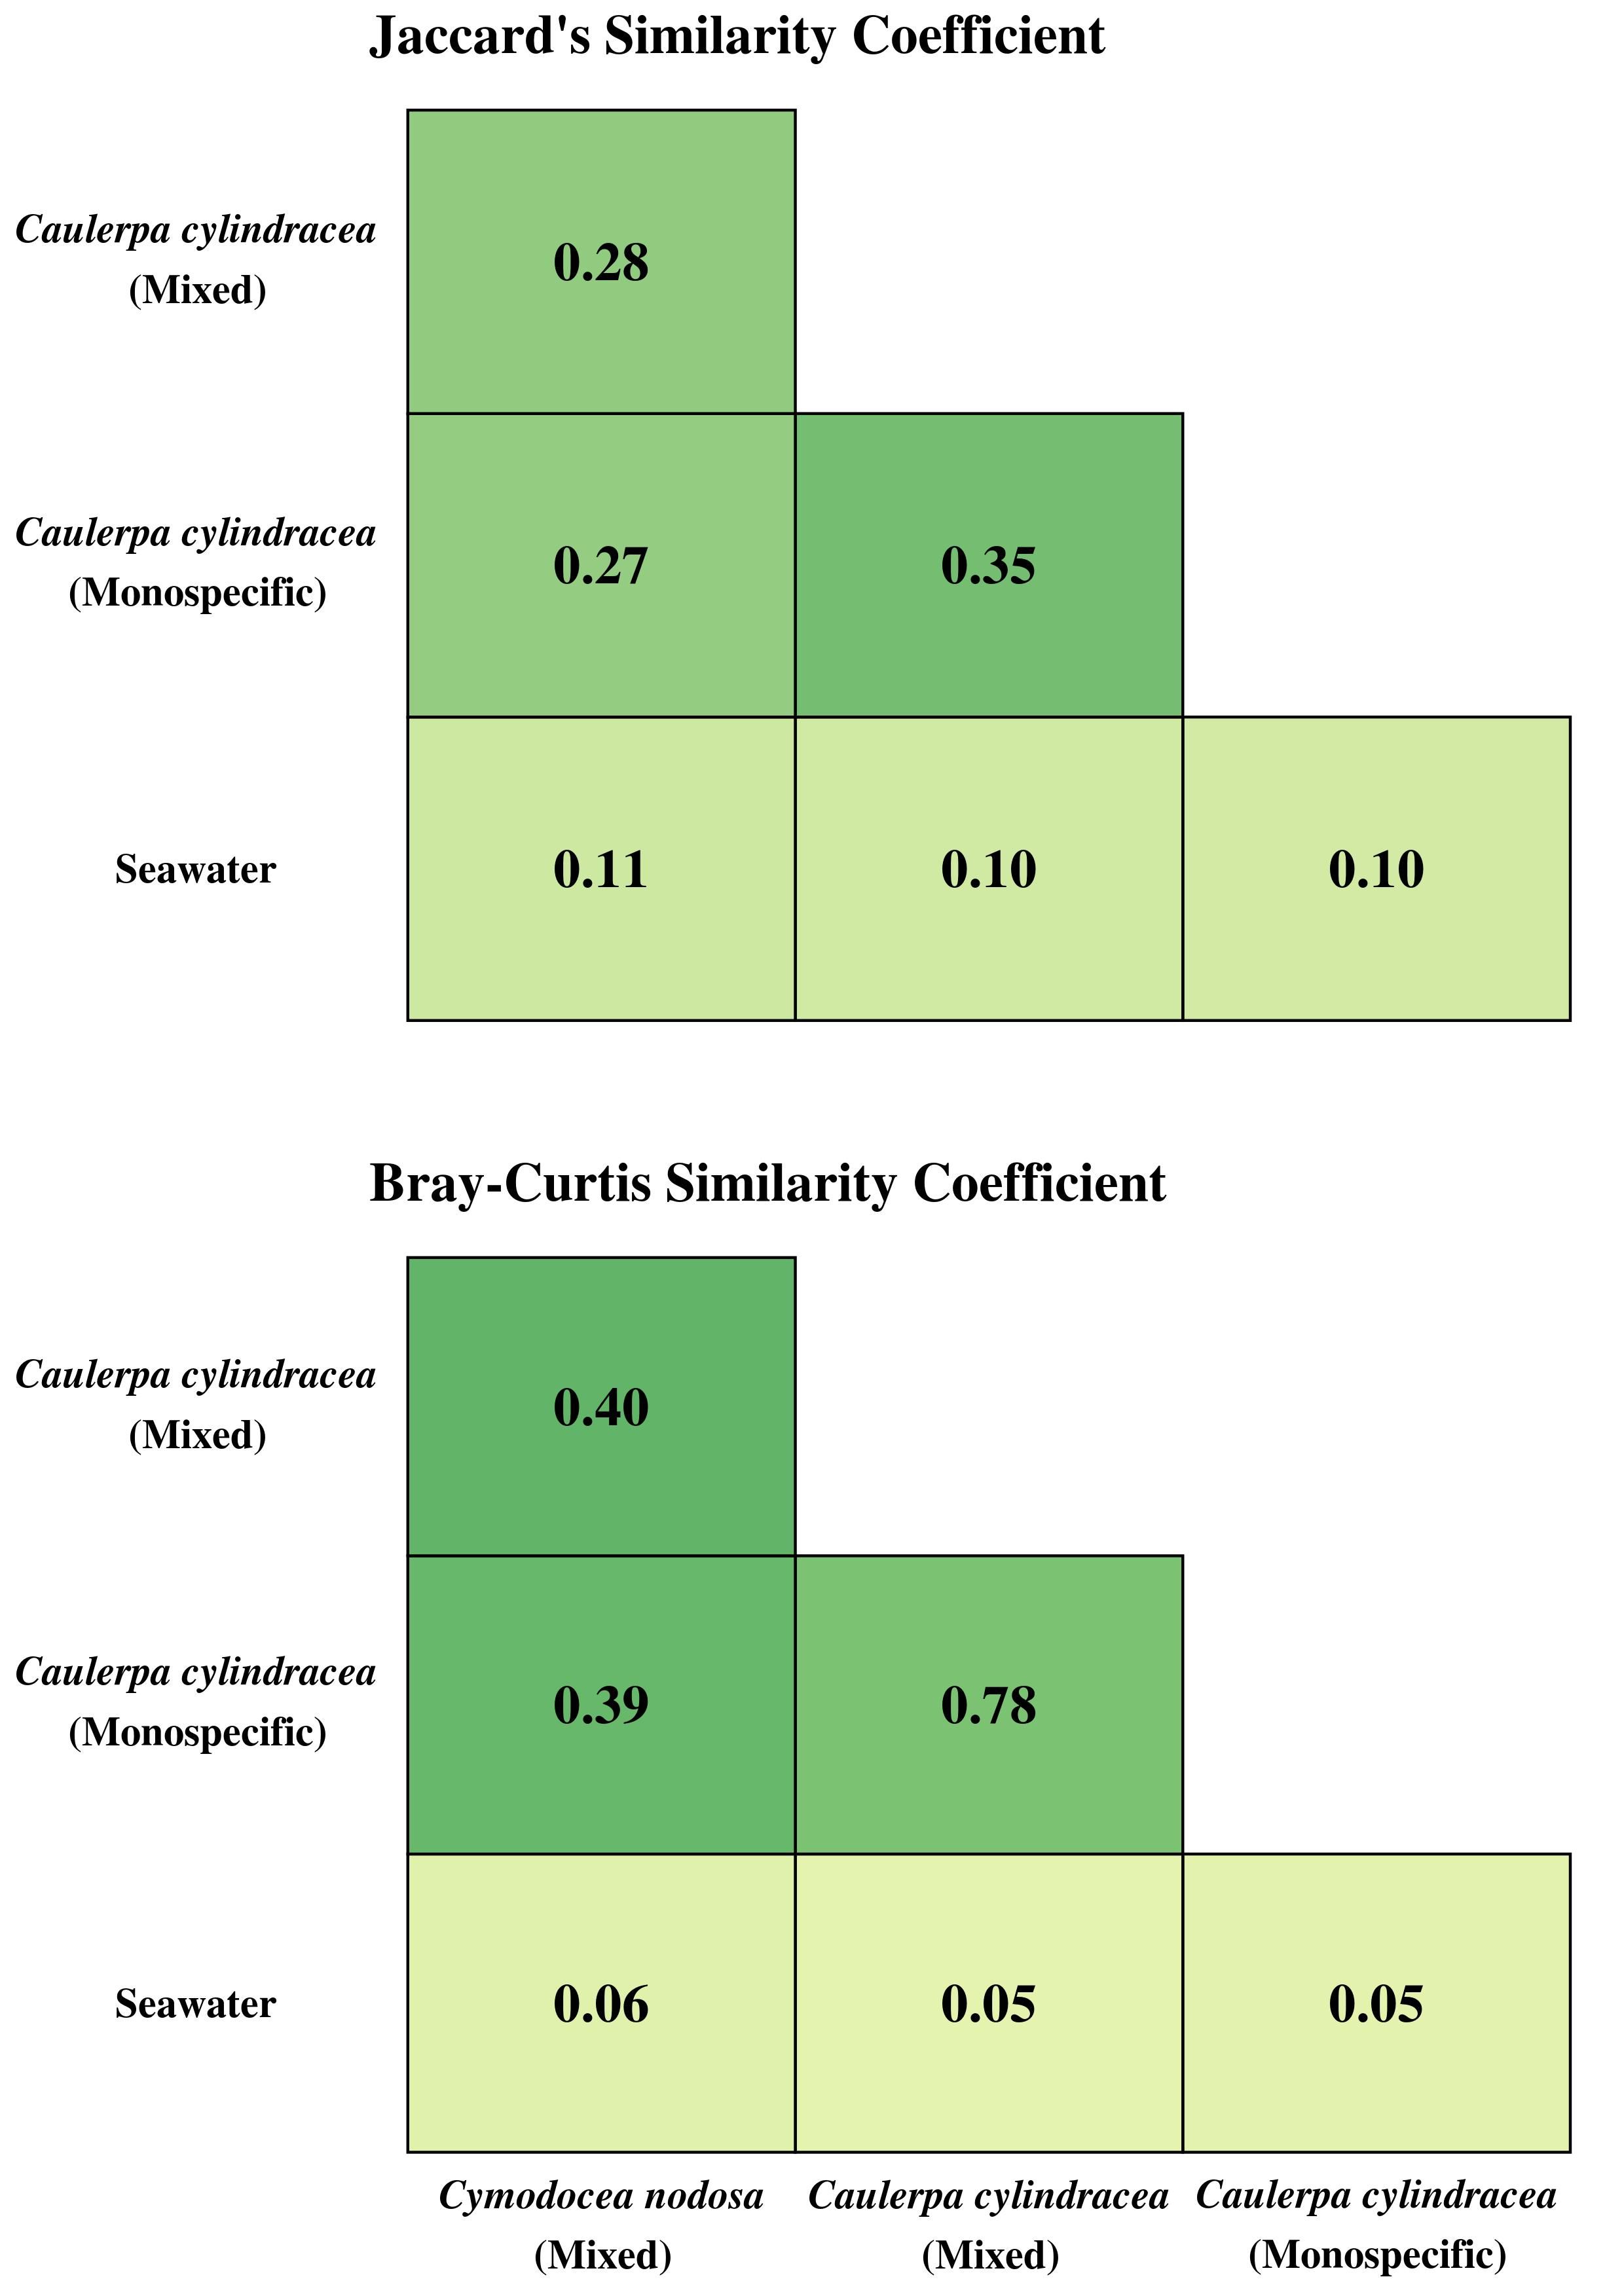
\includegraphics[width=0.7\linewidth]{../results/figures/matrix} 

}

\caption{Proportion of shared bacterial and archaeal OTUs (Jaccard's similarity coefficient) and shared bacterial and archaeal communities (Bray-Curtis similarity coefficient) between assemblages associated with the surfaces of the macrophytes \textit{C. nodosa} (mixed settlement) and \textit{C. cylindracea} (mixed and monospecific settlement) and communities in the ambient seawater.\label{matrix}}\label{fig:unnamed-chunk-1}
\end{figure}

\begin{figure}[H]

{\centering 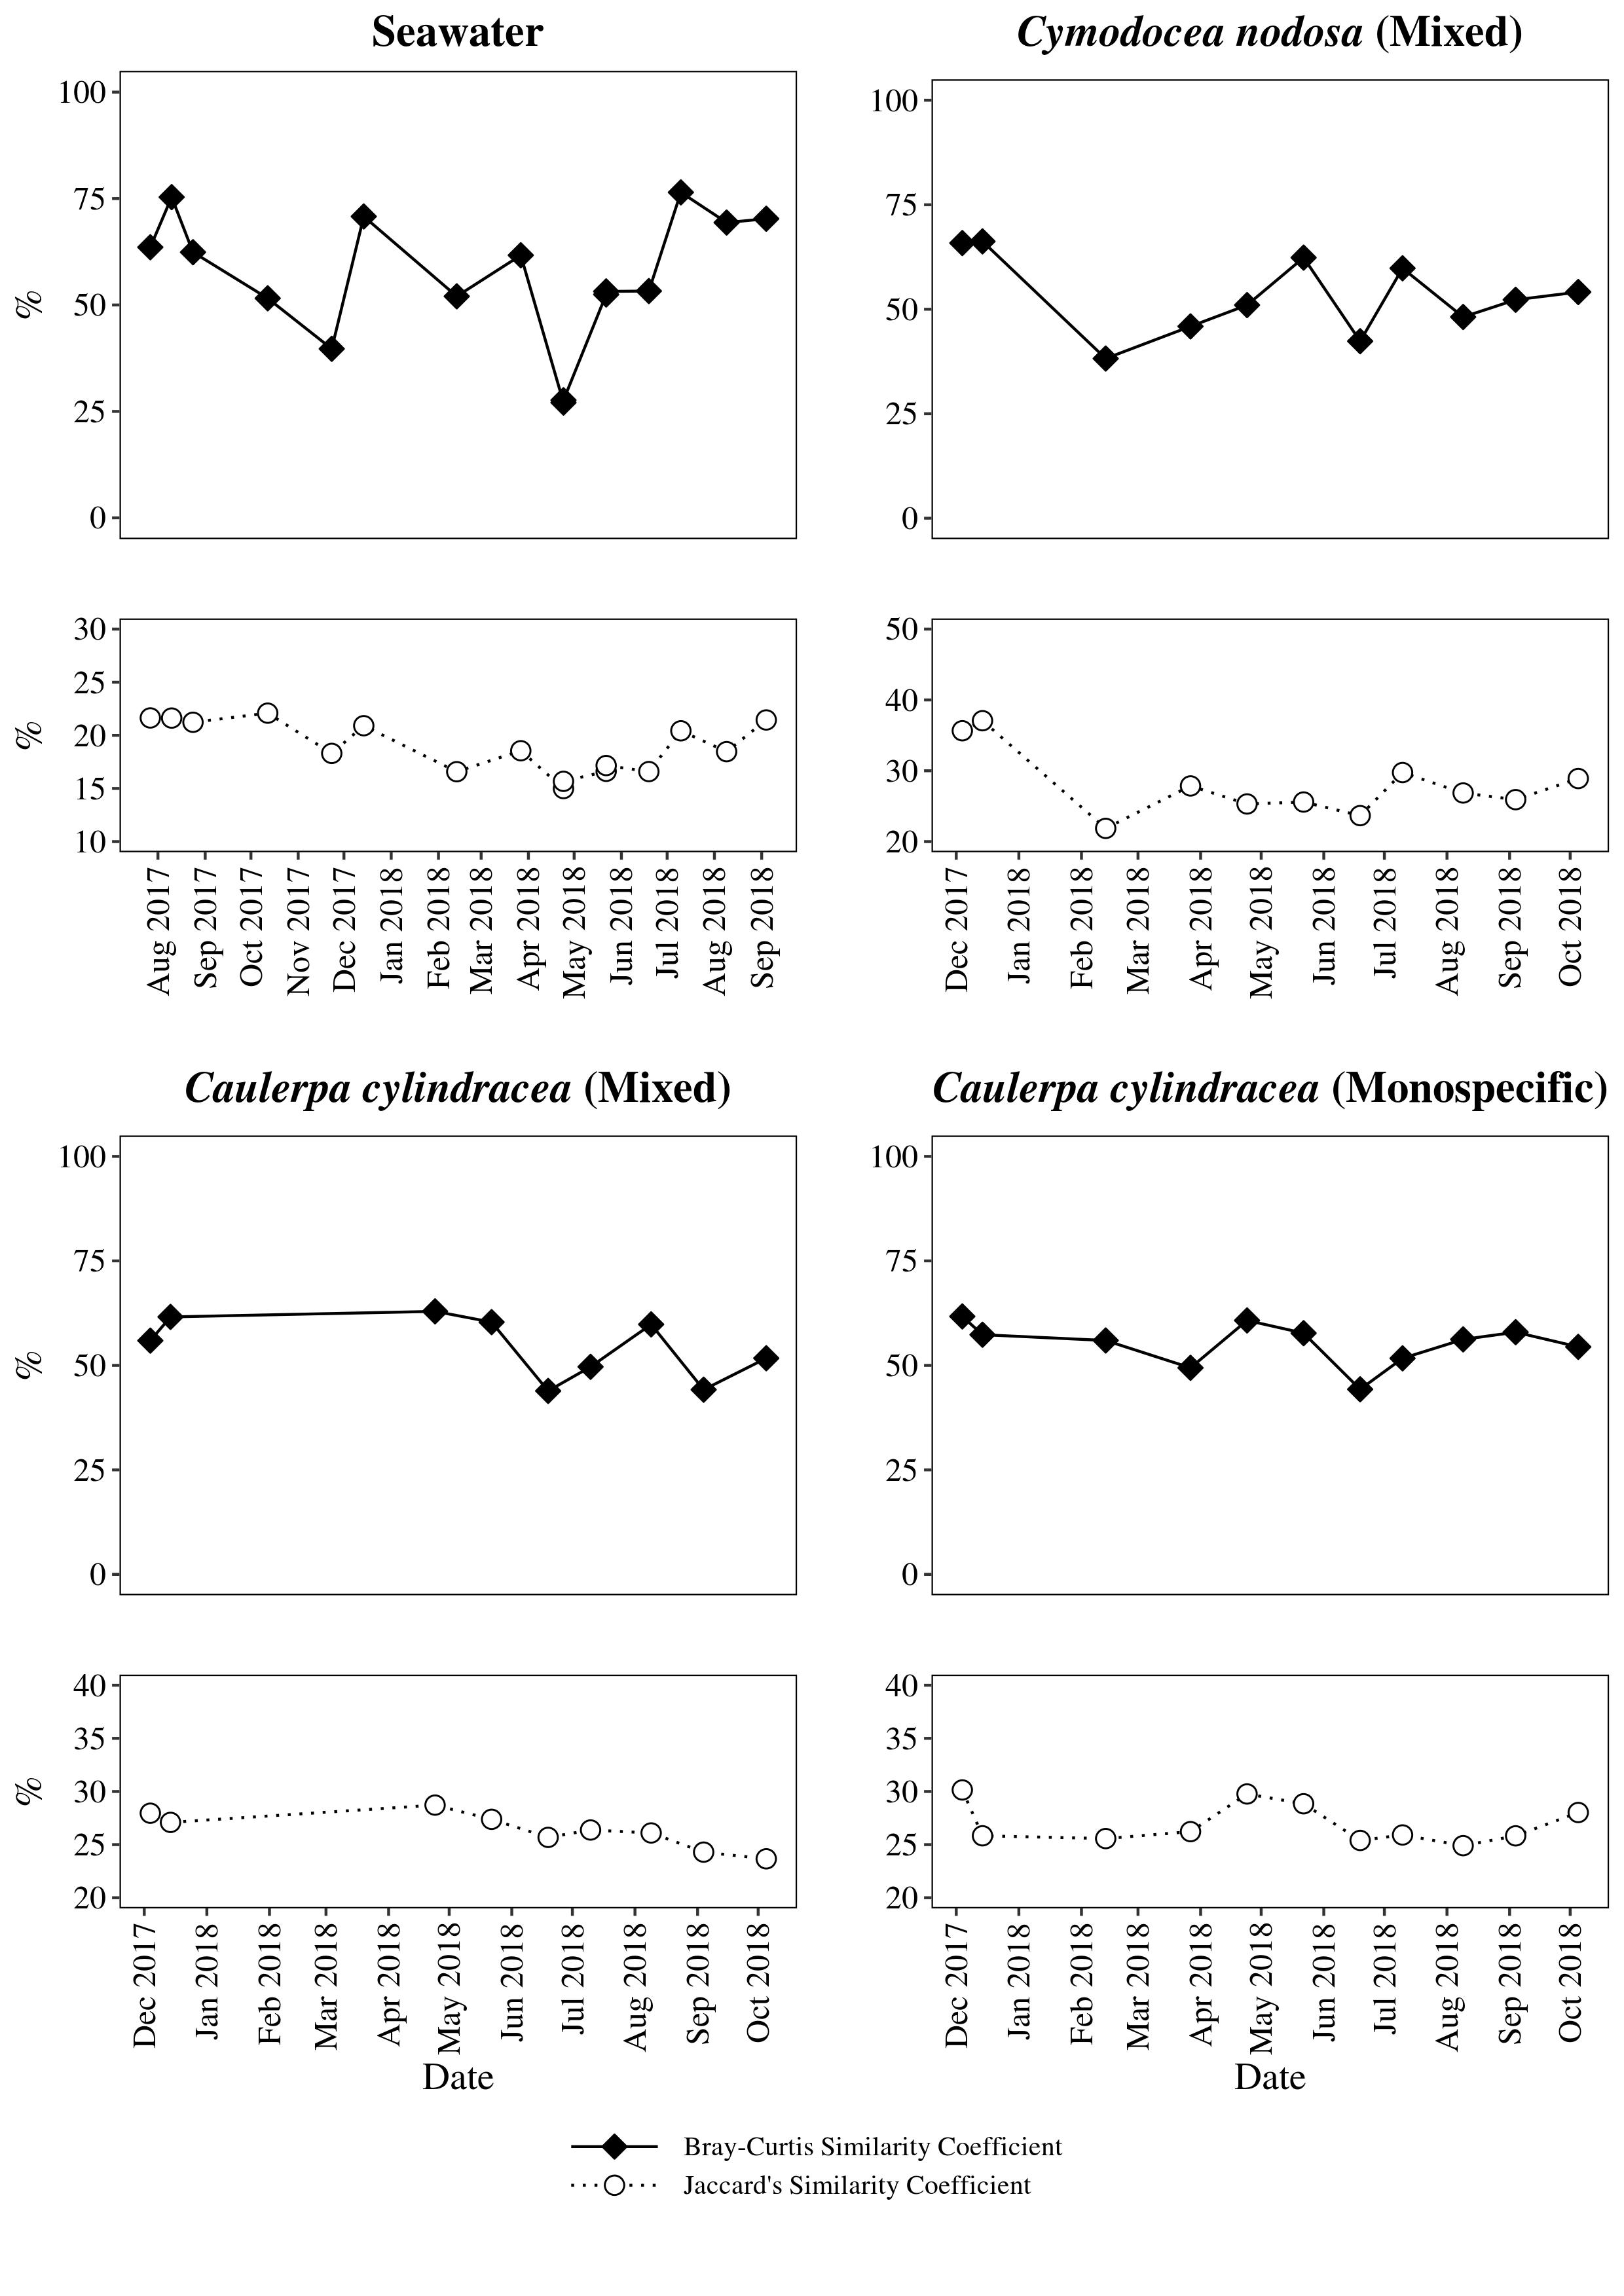
\includegraphics[width=0.85\linewidth]{../results/figures/seasonal_shared} 

}

\caption{Proportion of shared bacterial and archaeal communities (Bray-Curtis similarity coefficient) and shared bacterial and archaeal OTUs (Jaccard's similarity coefficient) between consecutive sampling dates and from the surfaces of the macrophytes \textit{C. nodosa} (mixed settlement) and \textit{C. cylindracea} (mixed and monospecific settlement) and in the ambient seawater.\label{shared}}\label{fig:unnamed-chunk-2}
\end{figure}

\begin{figure}[H]

{\centering 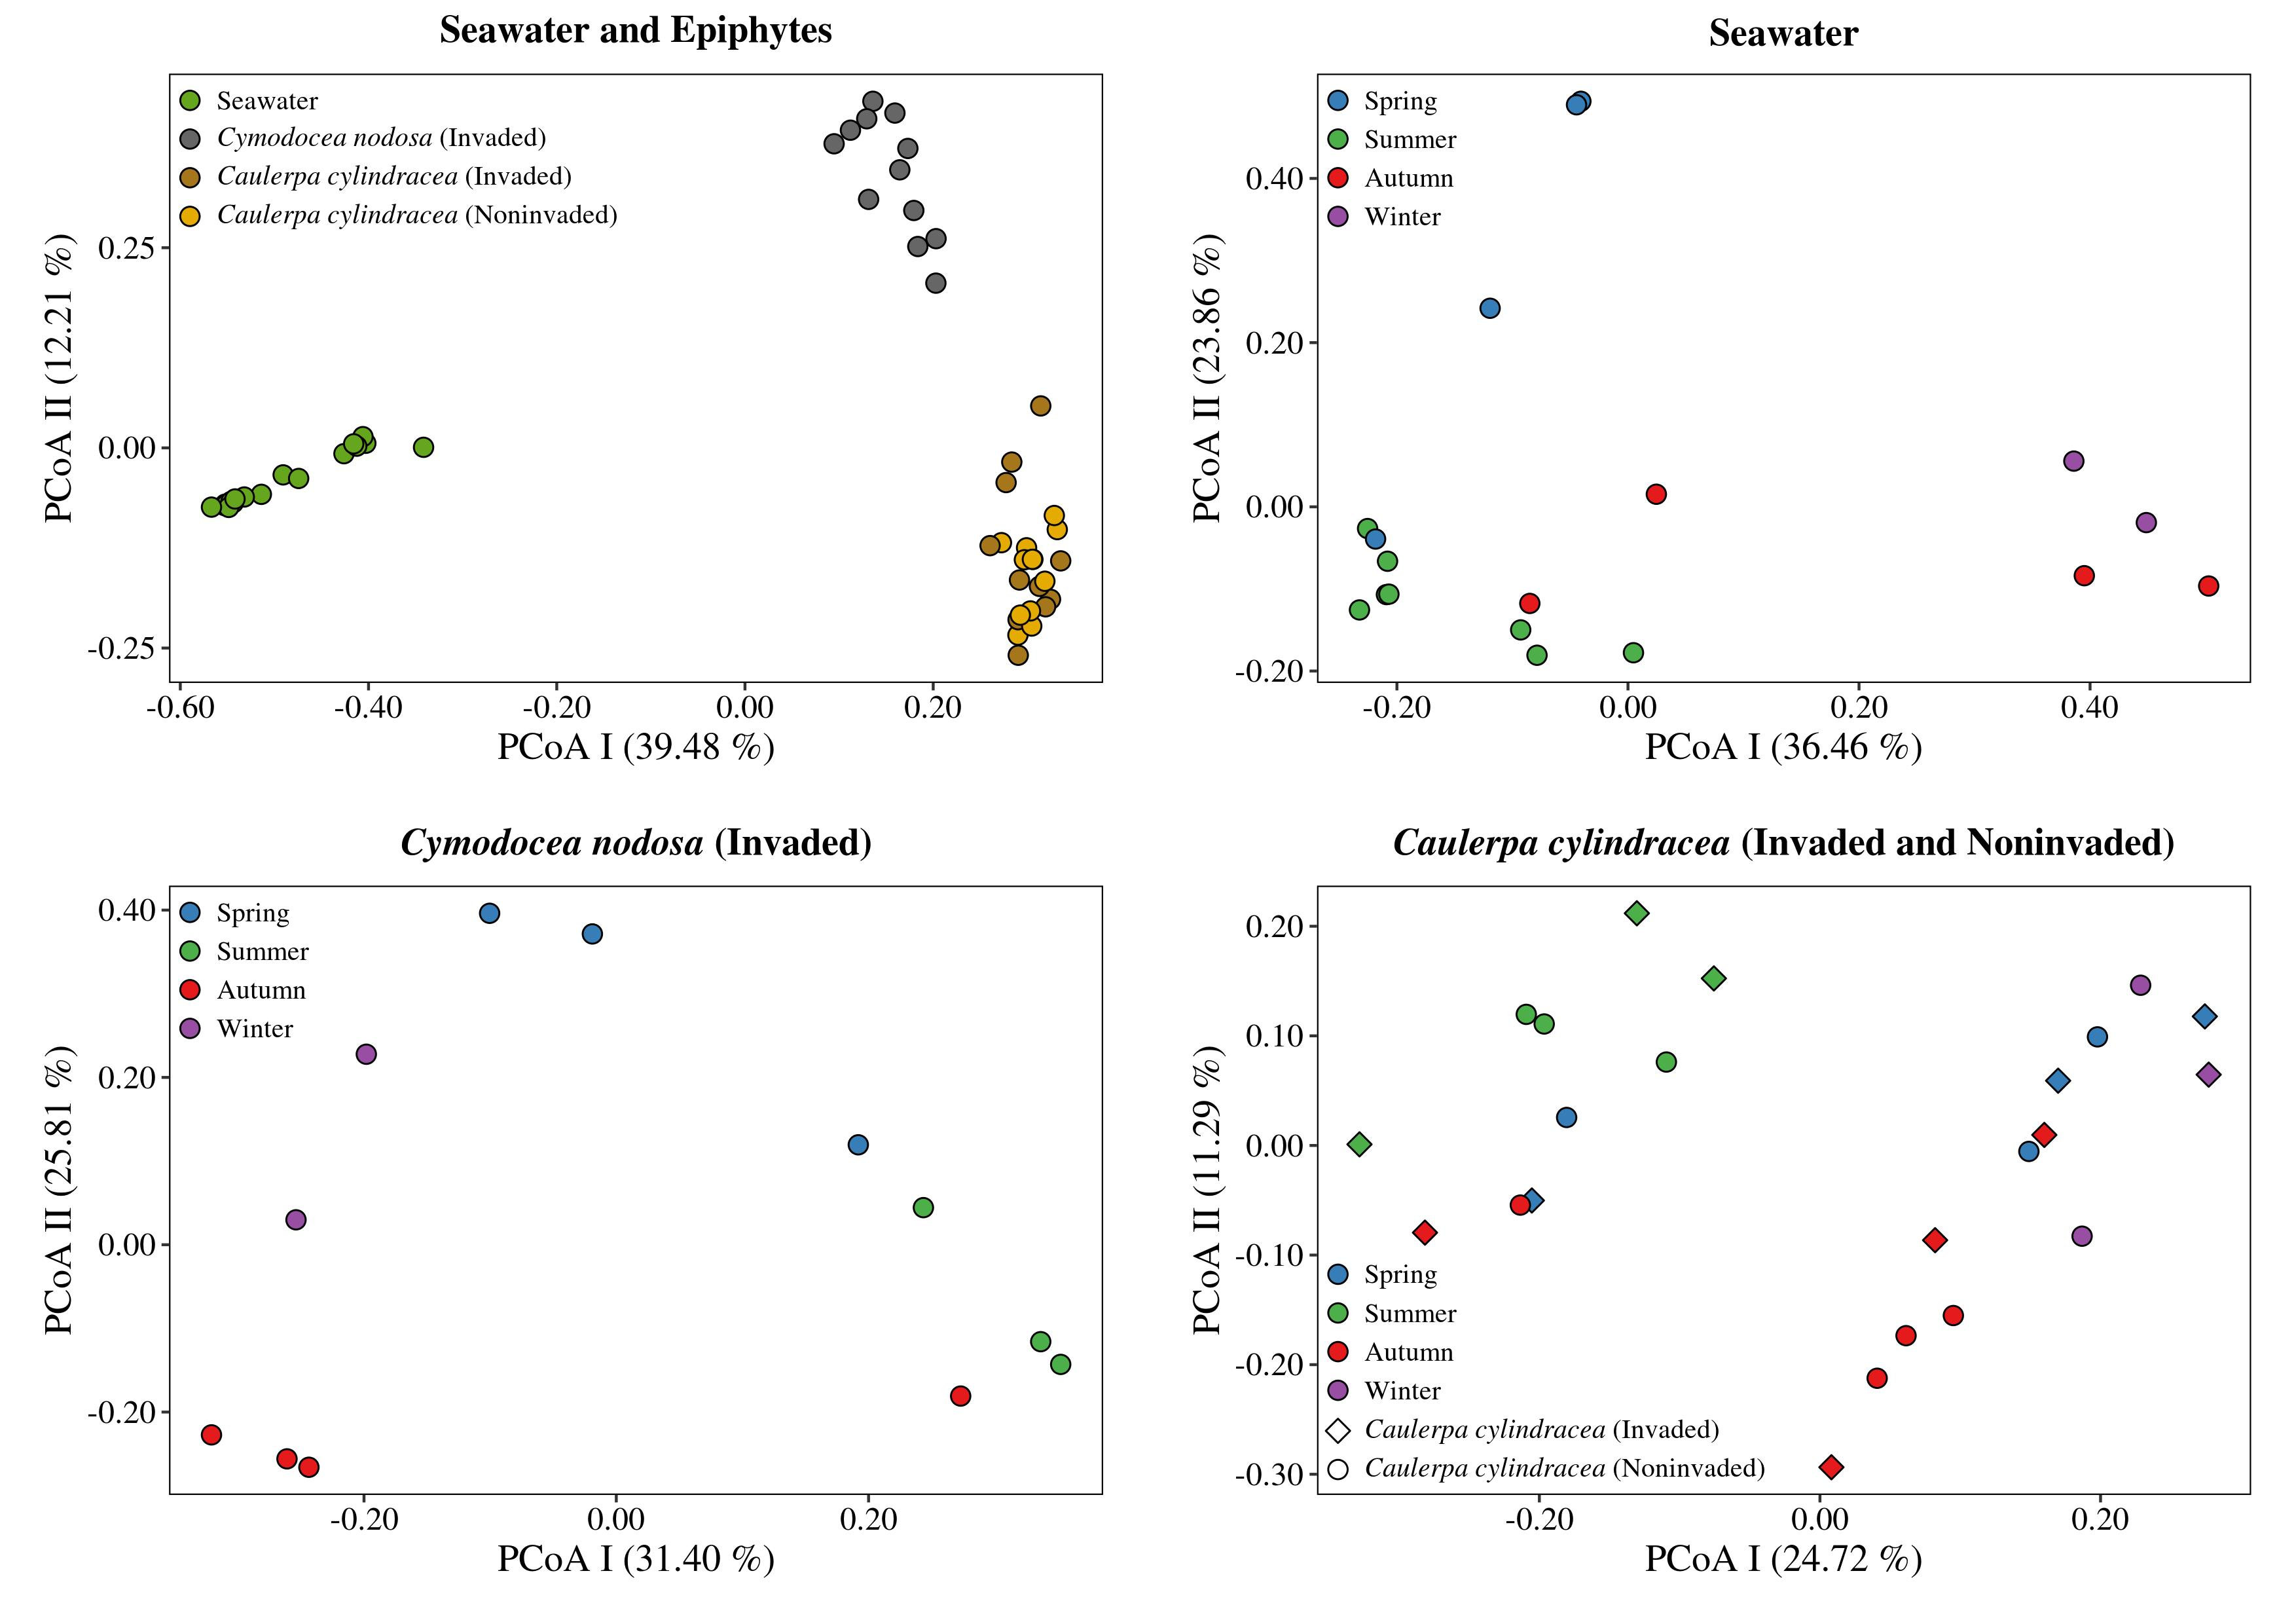
\includegraphics[width=0.55\linewidth]{../results/figures/pcoa_figure} 

}

\caption{Principal Coordinates Analysis (PCoA) of Bray-Curtis distances based on OTU abundances of bacterial and archaeal communities from the surfaces of the macrophytes \textit{C. nodosa} (mixed settlement) and \textit{C. cylindracea} (mixed and monospecific settlement) and in the ambient seawater. Samples from the same environment or same season are labeled in different colors. The proportion of explained variation by each axis is shown on the corresponding axis in parentheses.\label{pcoa}}\label{fig:unnamed-chunk-3}
\end{figure}

\begin{figure}[H]

{\centering 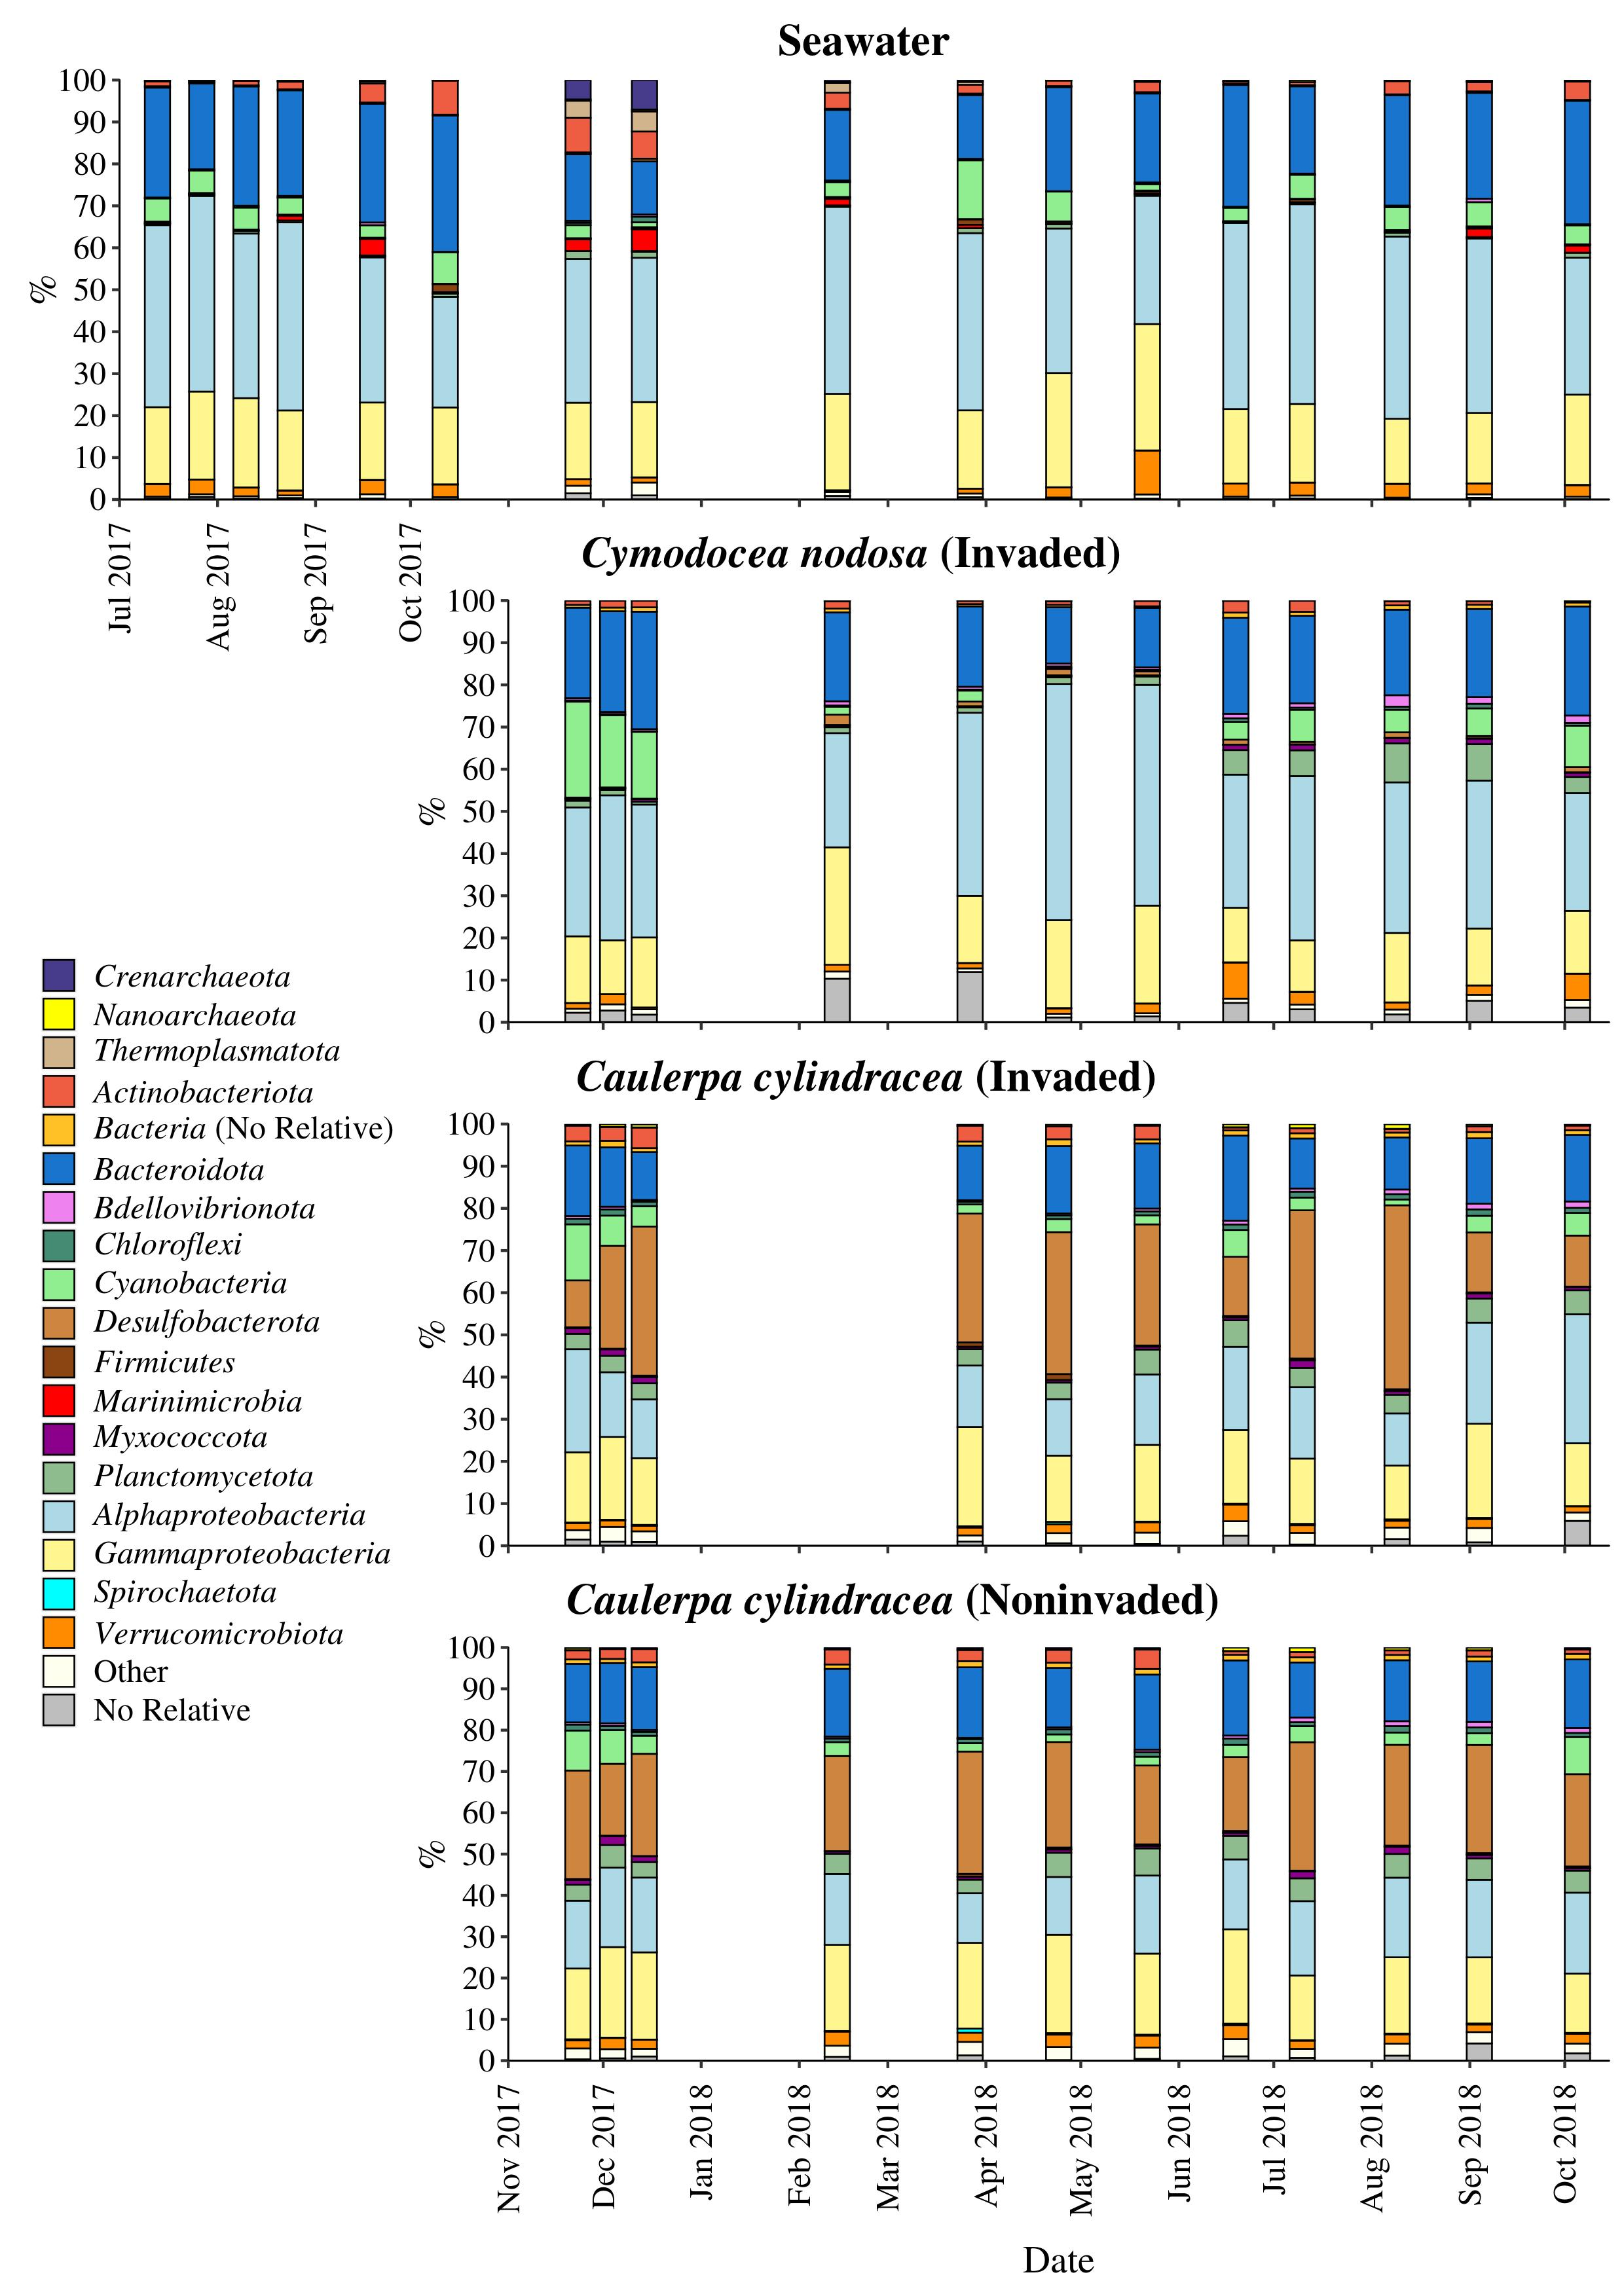
\includegraphics[width=0.85\linewidth]{../results/figures/community_bar_plot} 

}

\caption{Taxonomic classification and relative contribution of the most abundant (> 1 \si{\percent}) bacterial and archaeal sequences on the surfaces of the macrophytes \textit{C. nodosa} (mixed settlement) and \textit{C. cylindracea} (mixed and monospecific settlement) and in the ambient seawater. NR -- No Relative (sequences without known relatives within the corresponding group)\label{community}}\label{fig:unnamed-chunk-4}
\end{figure}

\begin{figure}[H]

{\centering 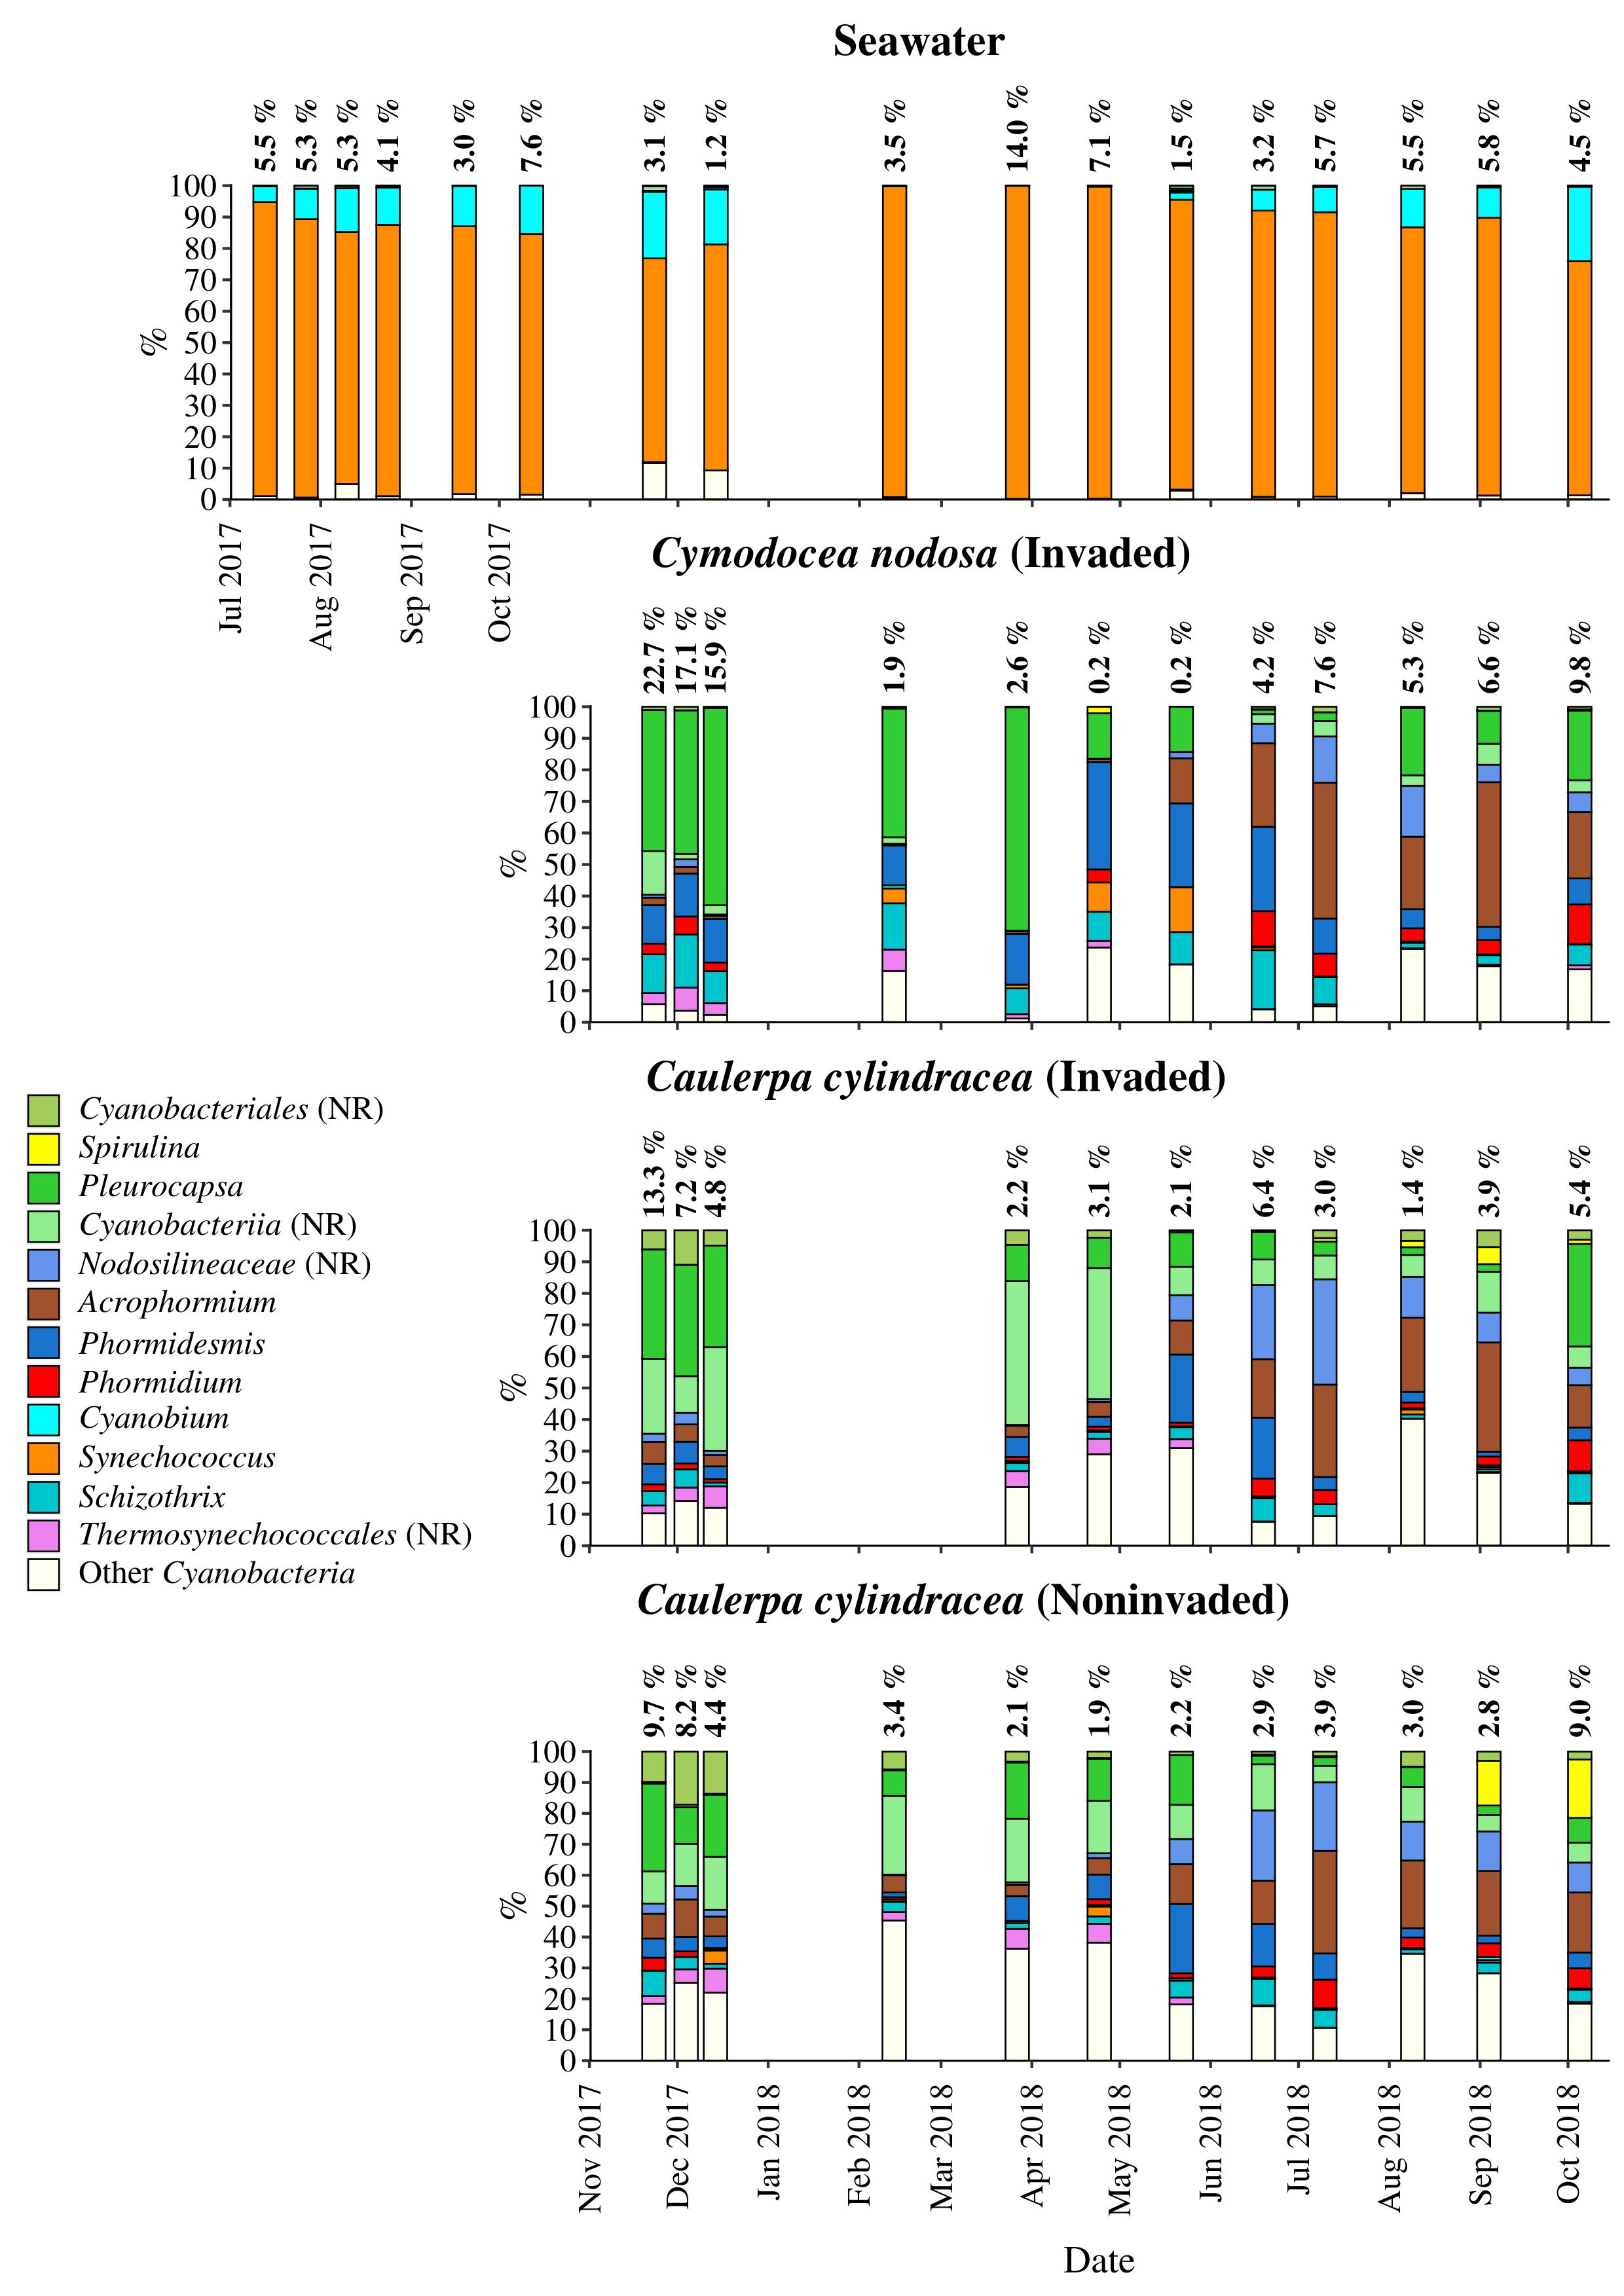
\includegraphics[width=0.85\linewidth]{../results/figures/cyanobacteria_bar_plot} 

}

\caption{Taxonomic classification and relative contribution of the most abundant (> 1 \si{\percent}) cyanobacterial sequences on the surfaces of the macrophytes \textit{C. nodosa} (mixed settlement) and \textit{C. cylindracea} (mixed and monospecific settlement) and in the ambient seawater. The proportion of cyanobacterial sequences in the total bacterial and archaeal community is given above the corresponding bar. NR -- No Relative (sequences without known relatives within the corresponding group)\label{cyano}}\label{fig:unnamed-chunk-5}
\end{figure}

\begin{figure}[H]

{\centering 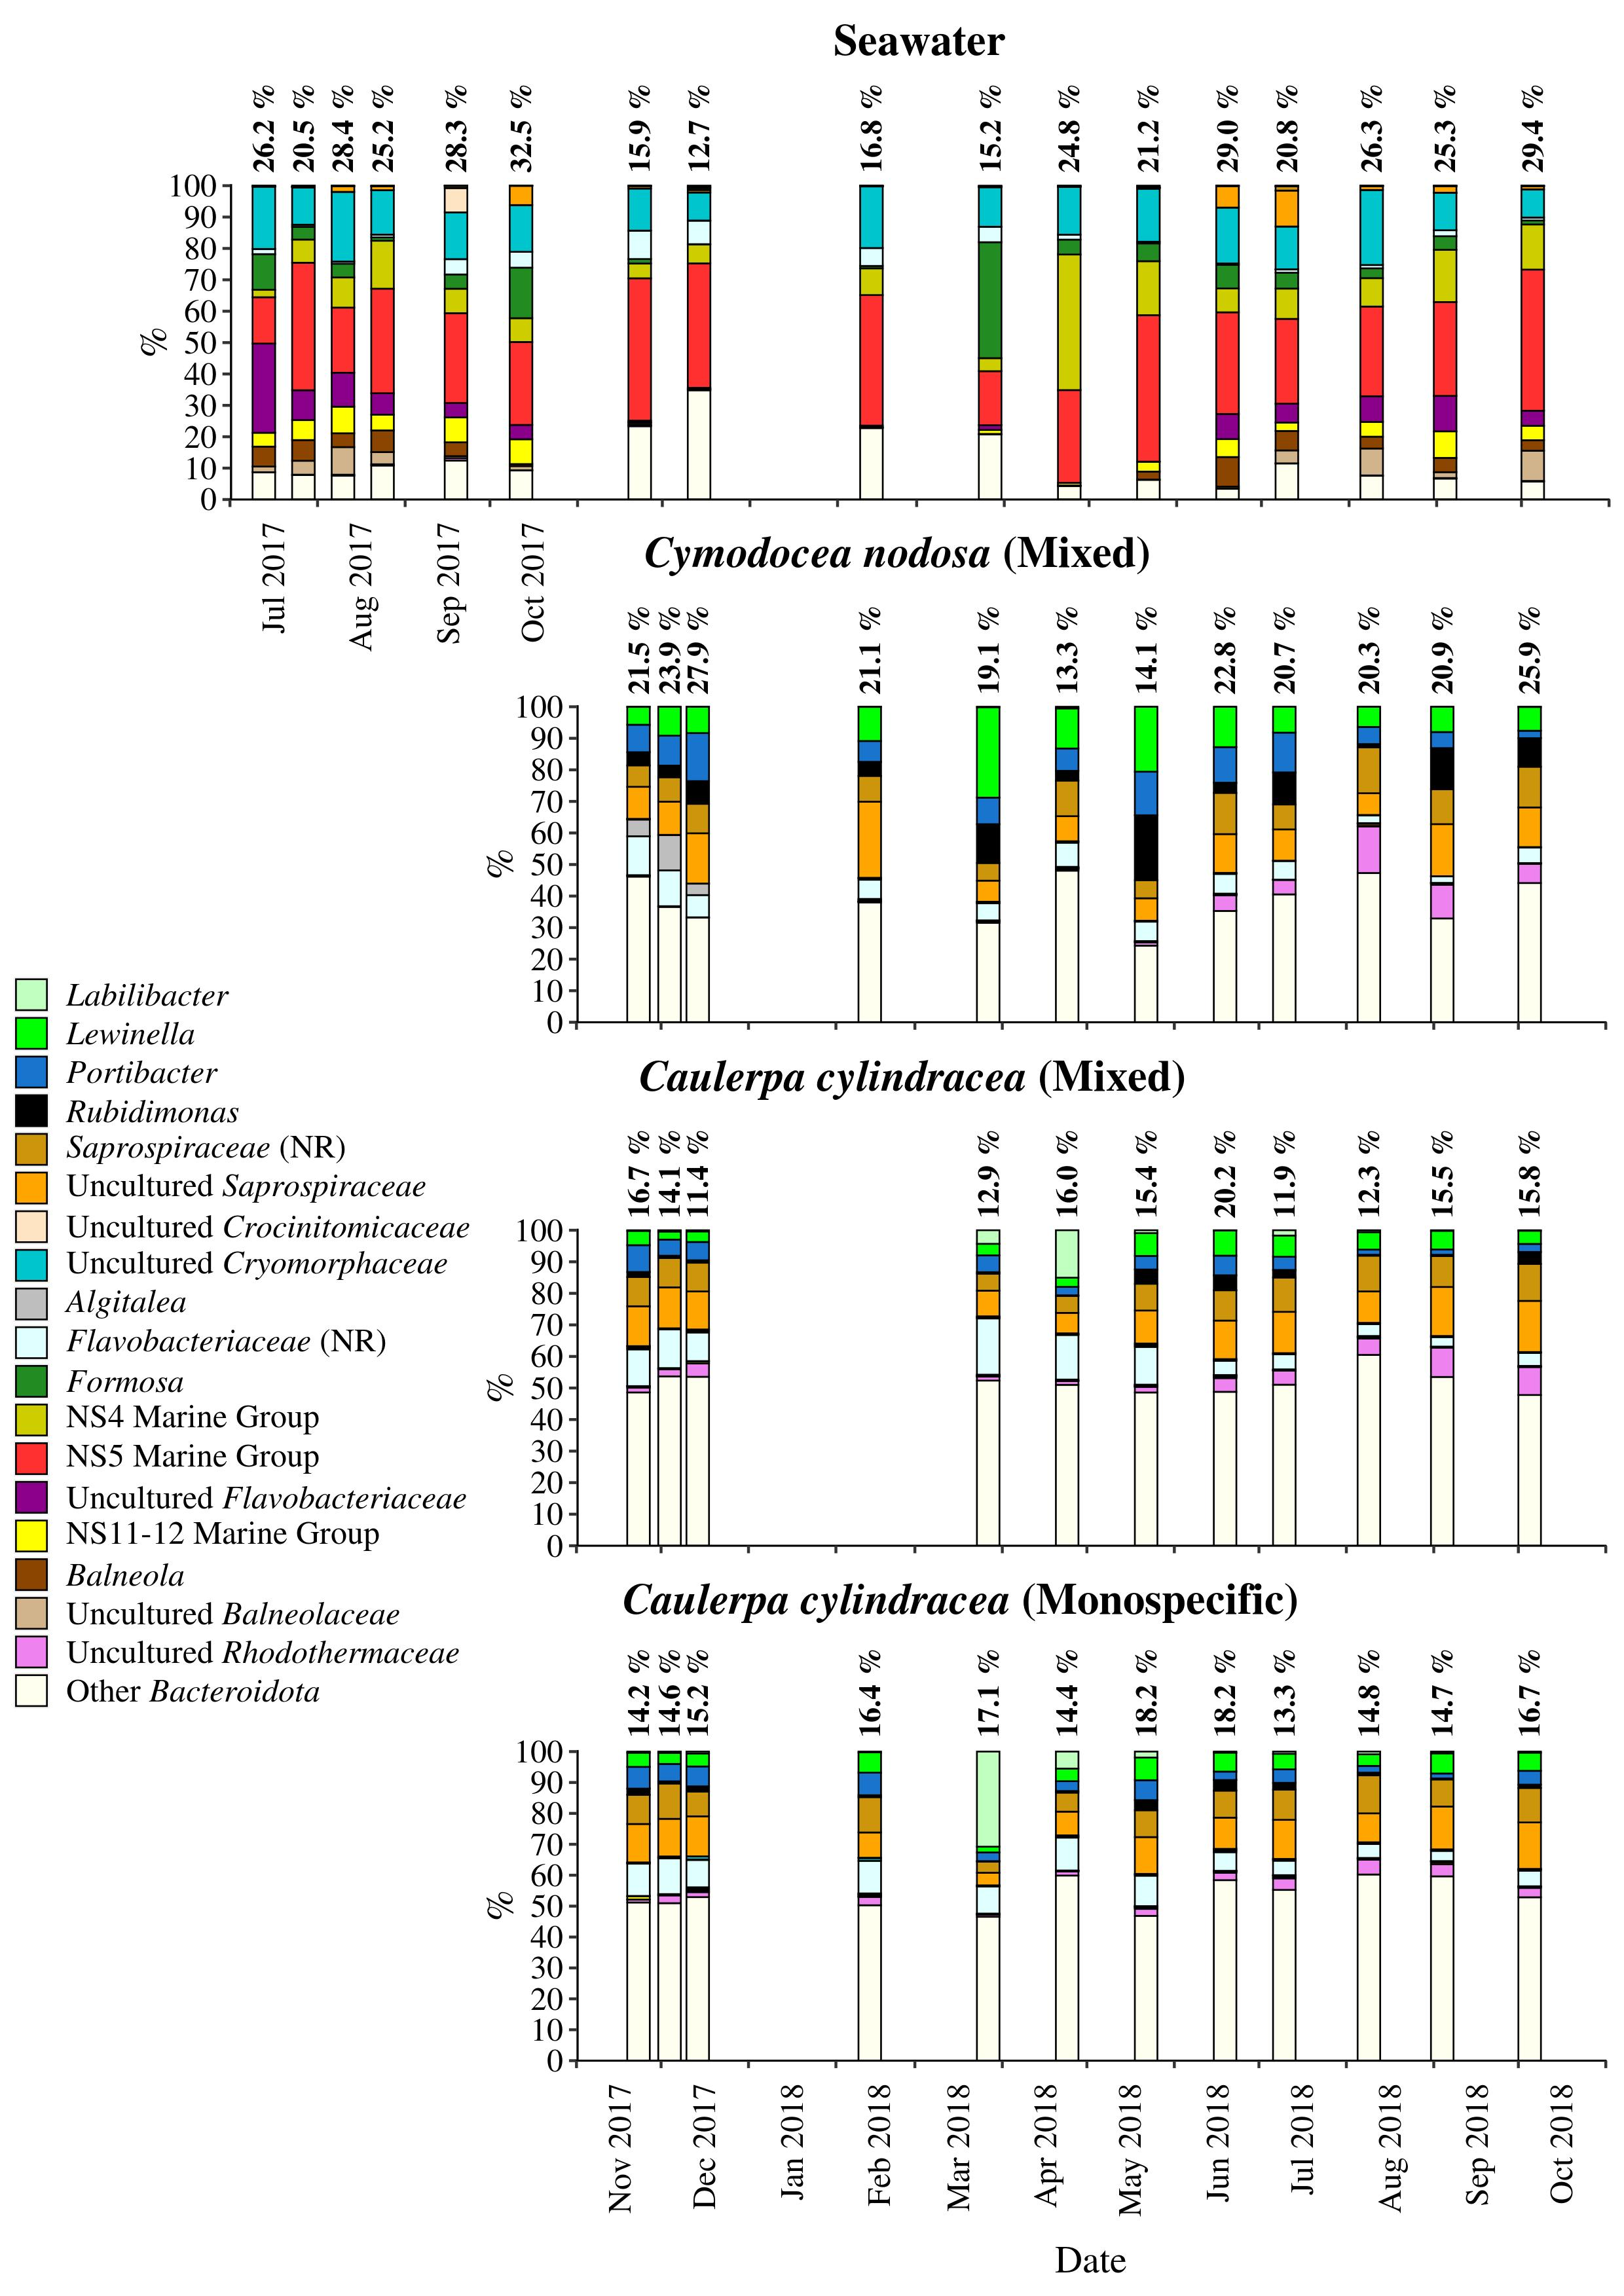
\includegraphics[width=0.85\linewidth]{../results/figures/bacteroidota_bar_plot} 

}

\caption{Taxonomic classification and relative contribution of the most abundant (> 2 \si{\percent}) sequences within the \textit{Bacteroidota} on the surfaces of the macrophytes \textit{C. nodosa} (mixed settlement) and \textit{C. cylindracea} (mixed and monospecific settlement) and in the ambient seawater. The proportion of sequences classified as \textit{Bacteroidota} in the total bacterial and archaeal community is given above the corresponding bar. NR -- No Relative (sequences without known relatives within the corresponding group)\label{bactero}}\label{fig:unnamed-chunk-6}
\end{figure}

\begin{figure}[H]

{\centering 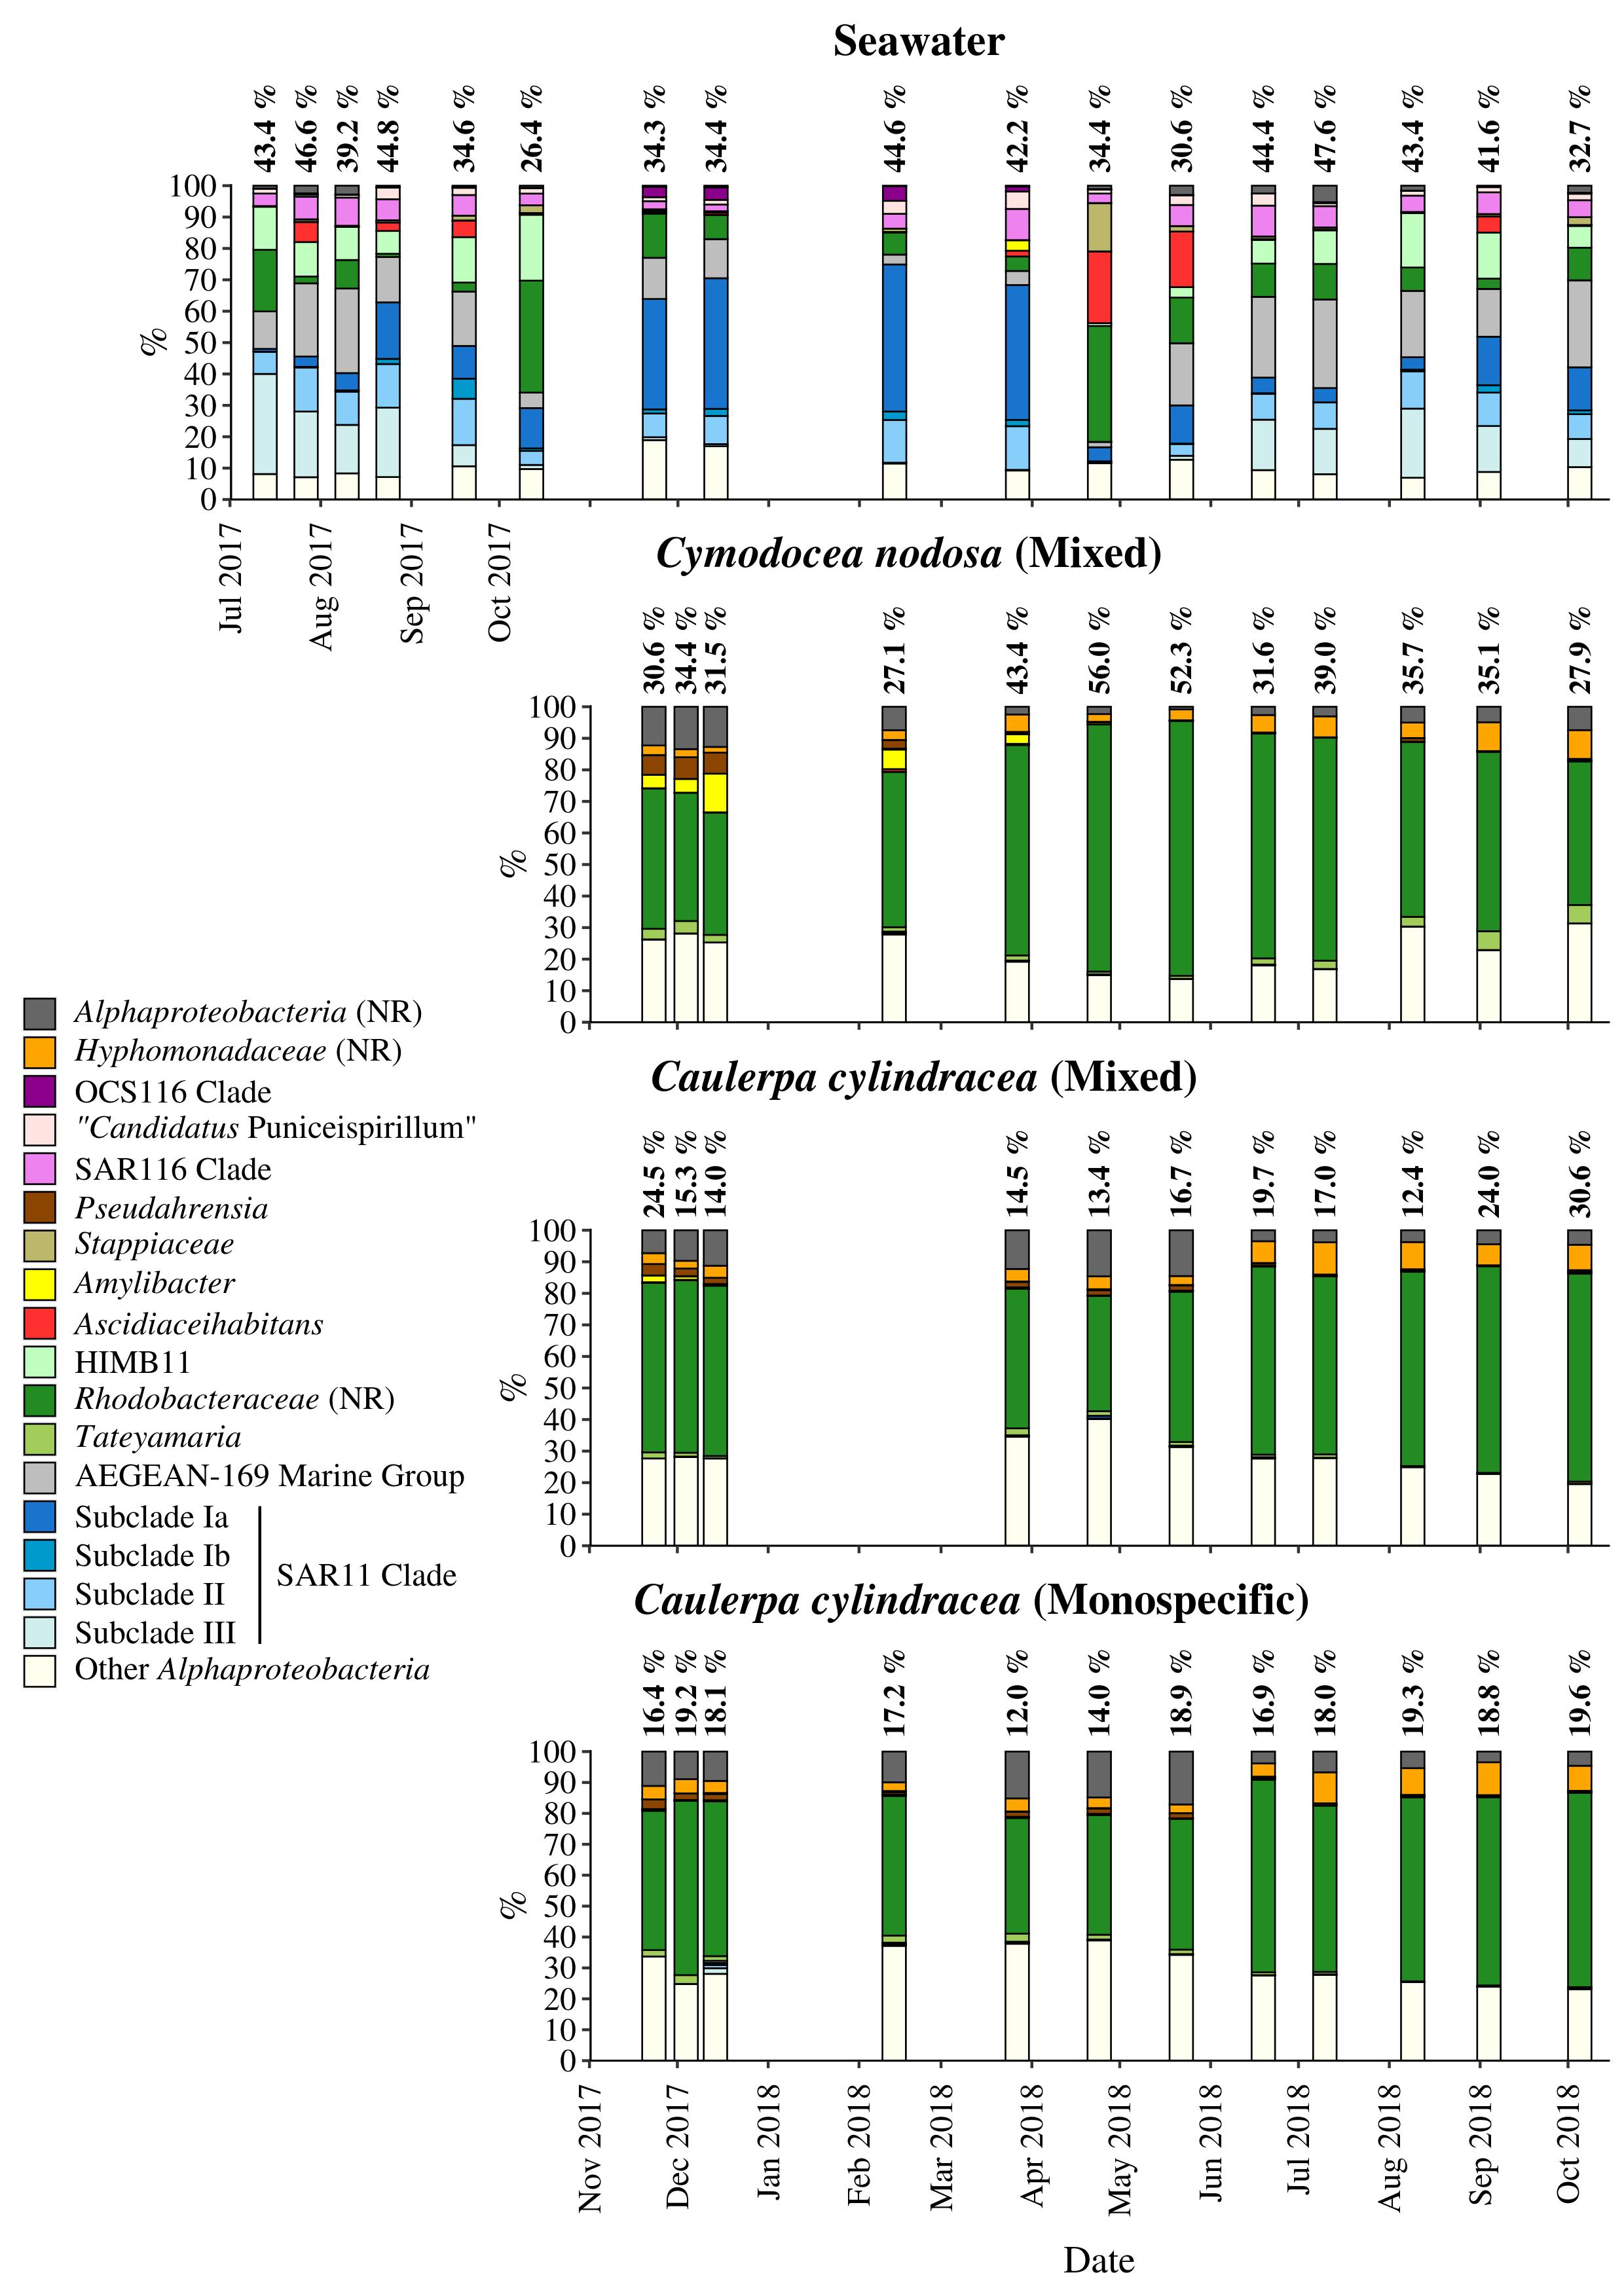
\includegraphics[width=0.85\linewidth]{../results/figures/alphaproteobacteria_bar_plot} 

}

\caption{Taxonomic classification and relative contribution of the most abundant (> 2 \si{\percent}) alphaproteobacterial sequences on the surfaces of the macrophytes \textit{C. nodosa} (mixed settlement) and \textit{C. cylindracea} (mixed and monospecific settlement) and in the ambient seawater. The proportion of alphaproteobacterial sequences in the total bacterial and archaeal community is given above the corresponding bar. NR -- No Relative (sequences without known relatives within the corresponding group)\label{alpha}}\label{fig:unnamed-chunk-7}
\end{figure}

\begin{figure}[H]

{\centering 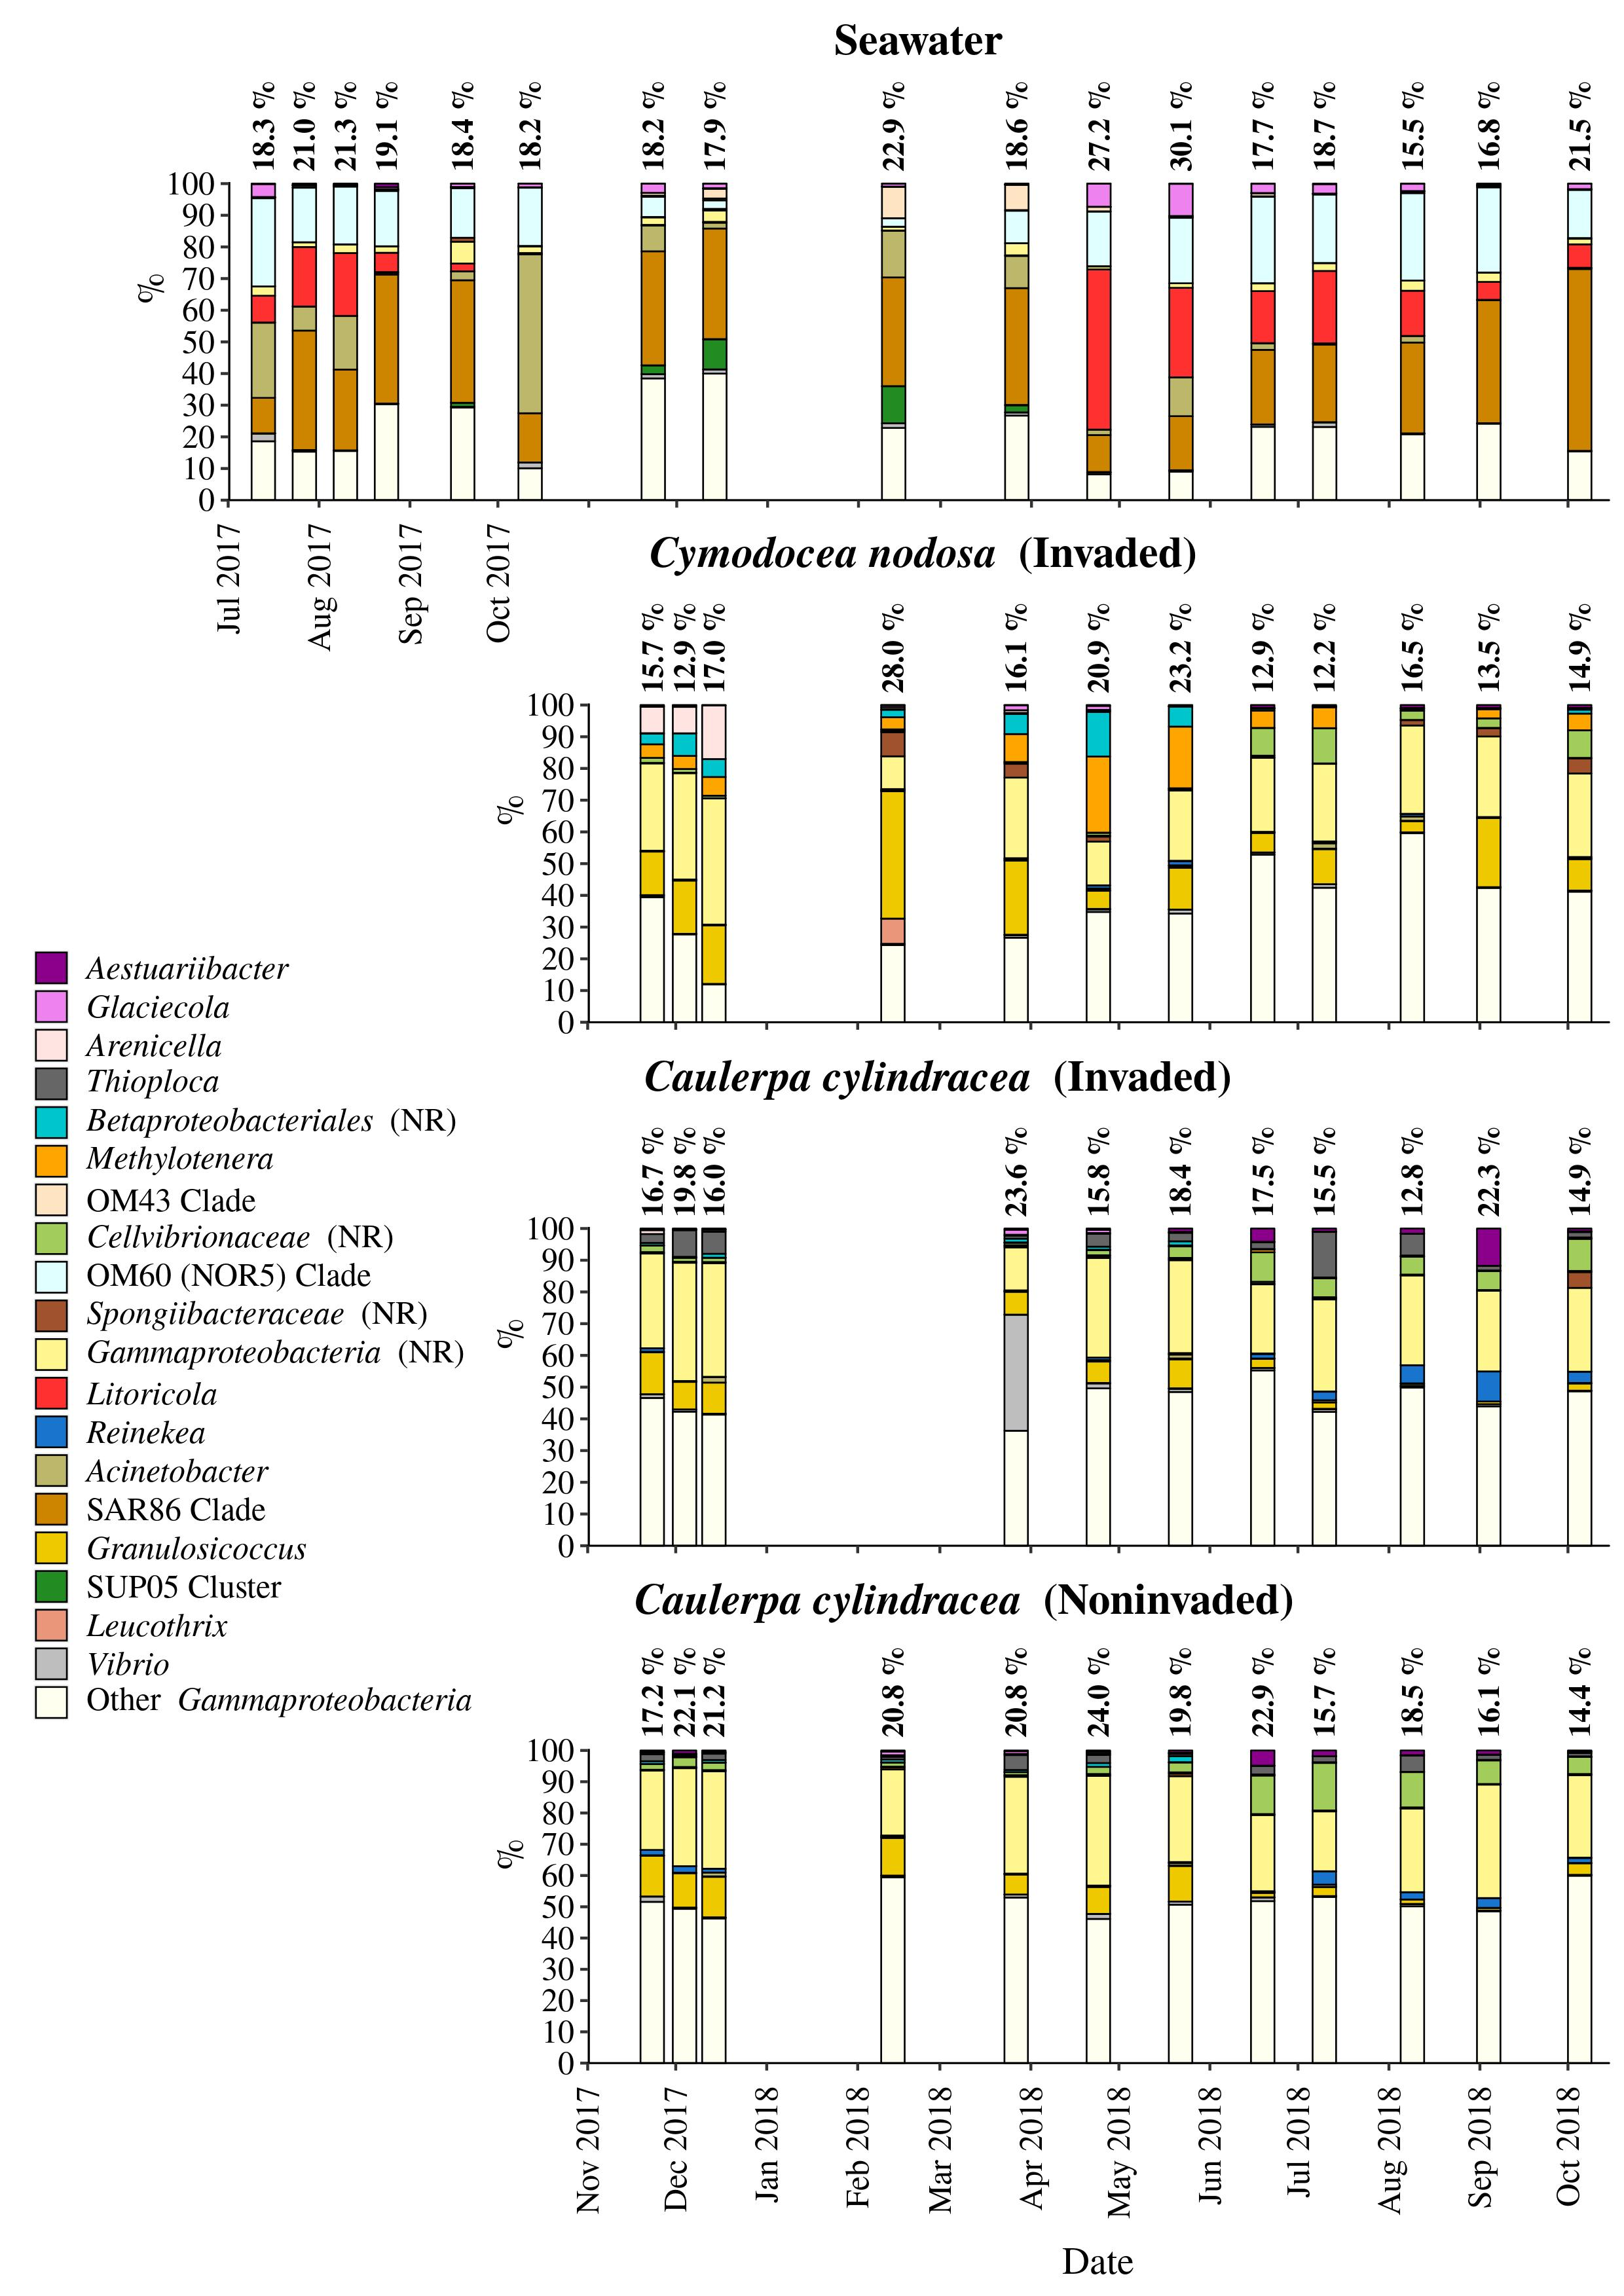
\includegraphics[width=0.85\linewidth]{../results/figures/gammaproteobacteria_bar_plot} 

}

\caption{Taxonomic classification and relative contribution of the most abundant (> 2 \si{\percent}) gammaproteobacterial sequences on the surfaces of the macrophytes \textit{C. nodosa} (mixed settlement) and \textit{C. cylindracea} (mixed and monospecific settlement) and in the ambient seawater. The proportion of gammaproteobacterial sequences in the total bacterial and archaeal community is given above the corresponding bar. NR -- No Relative (sequences without known relatives within the corresponding group)\label{gamma}}\label{fig:unnamed-chunk-8}
\end{figure}

\begin{figure}[H]

{\centering 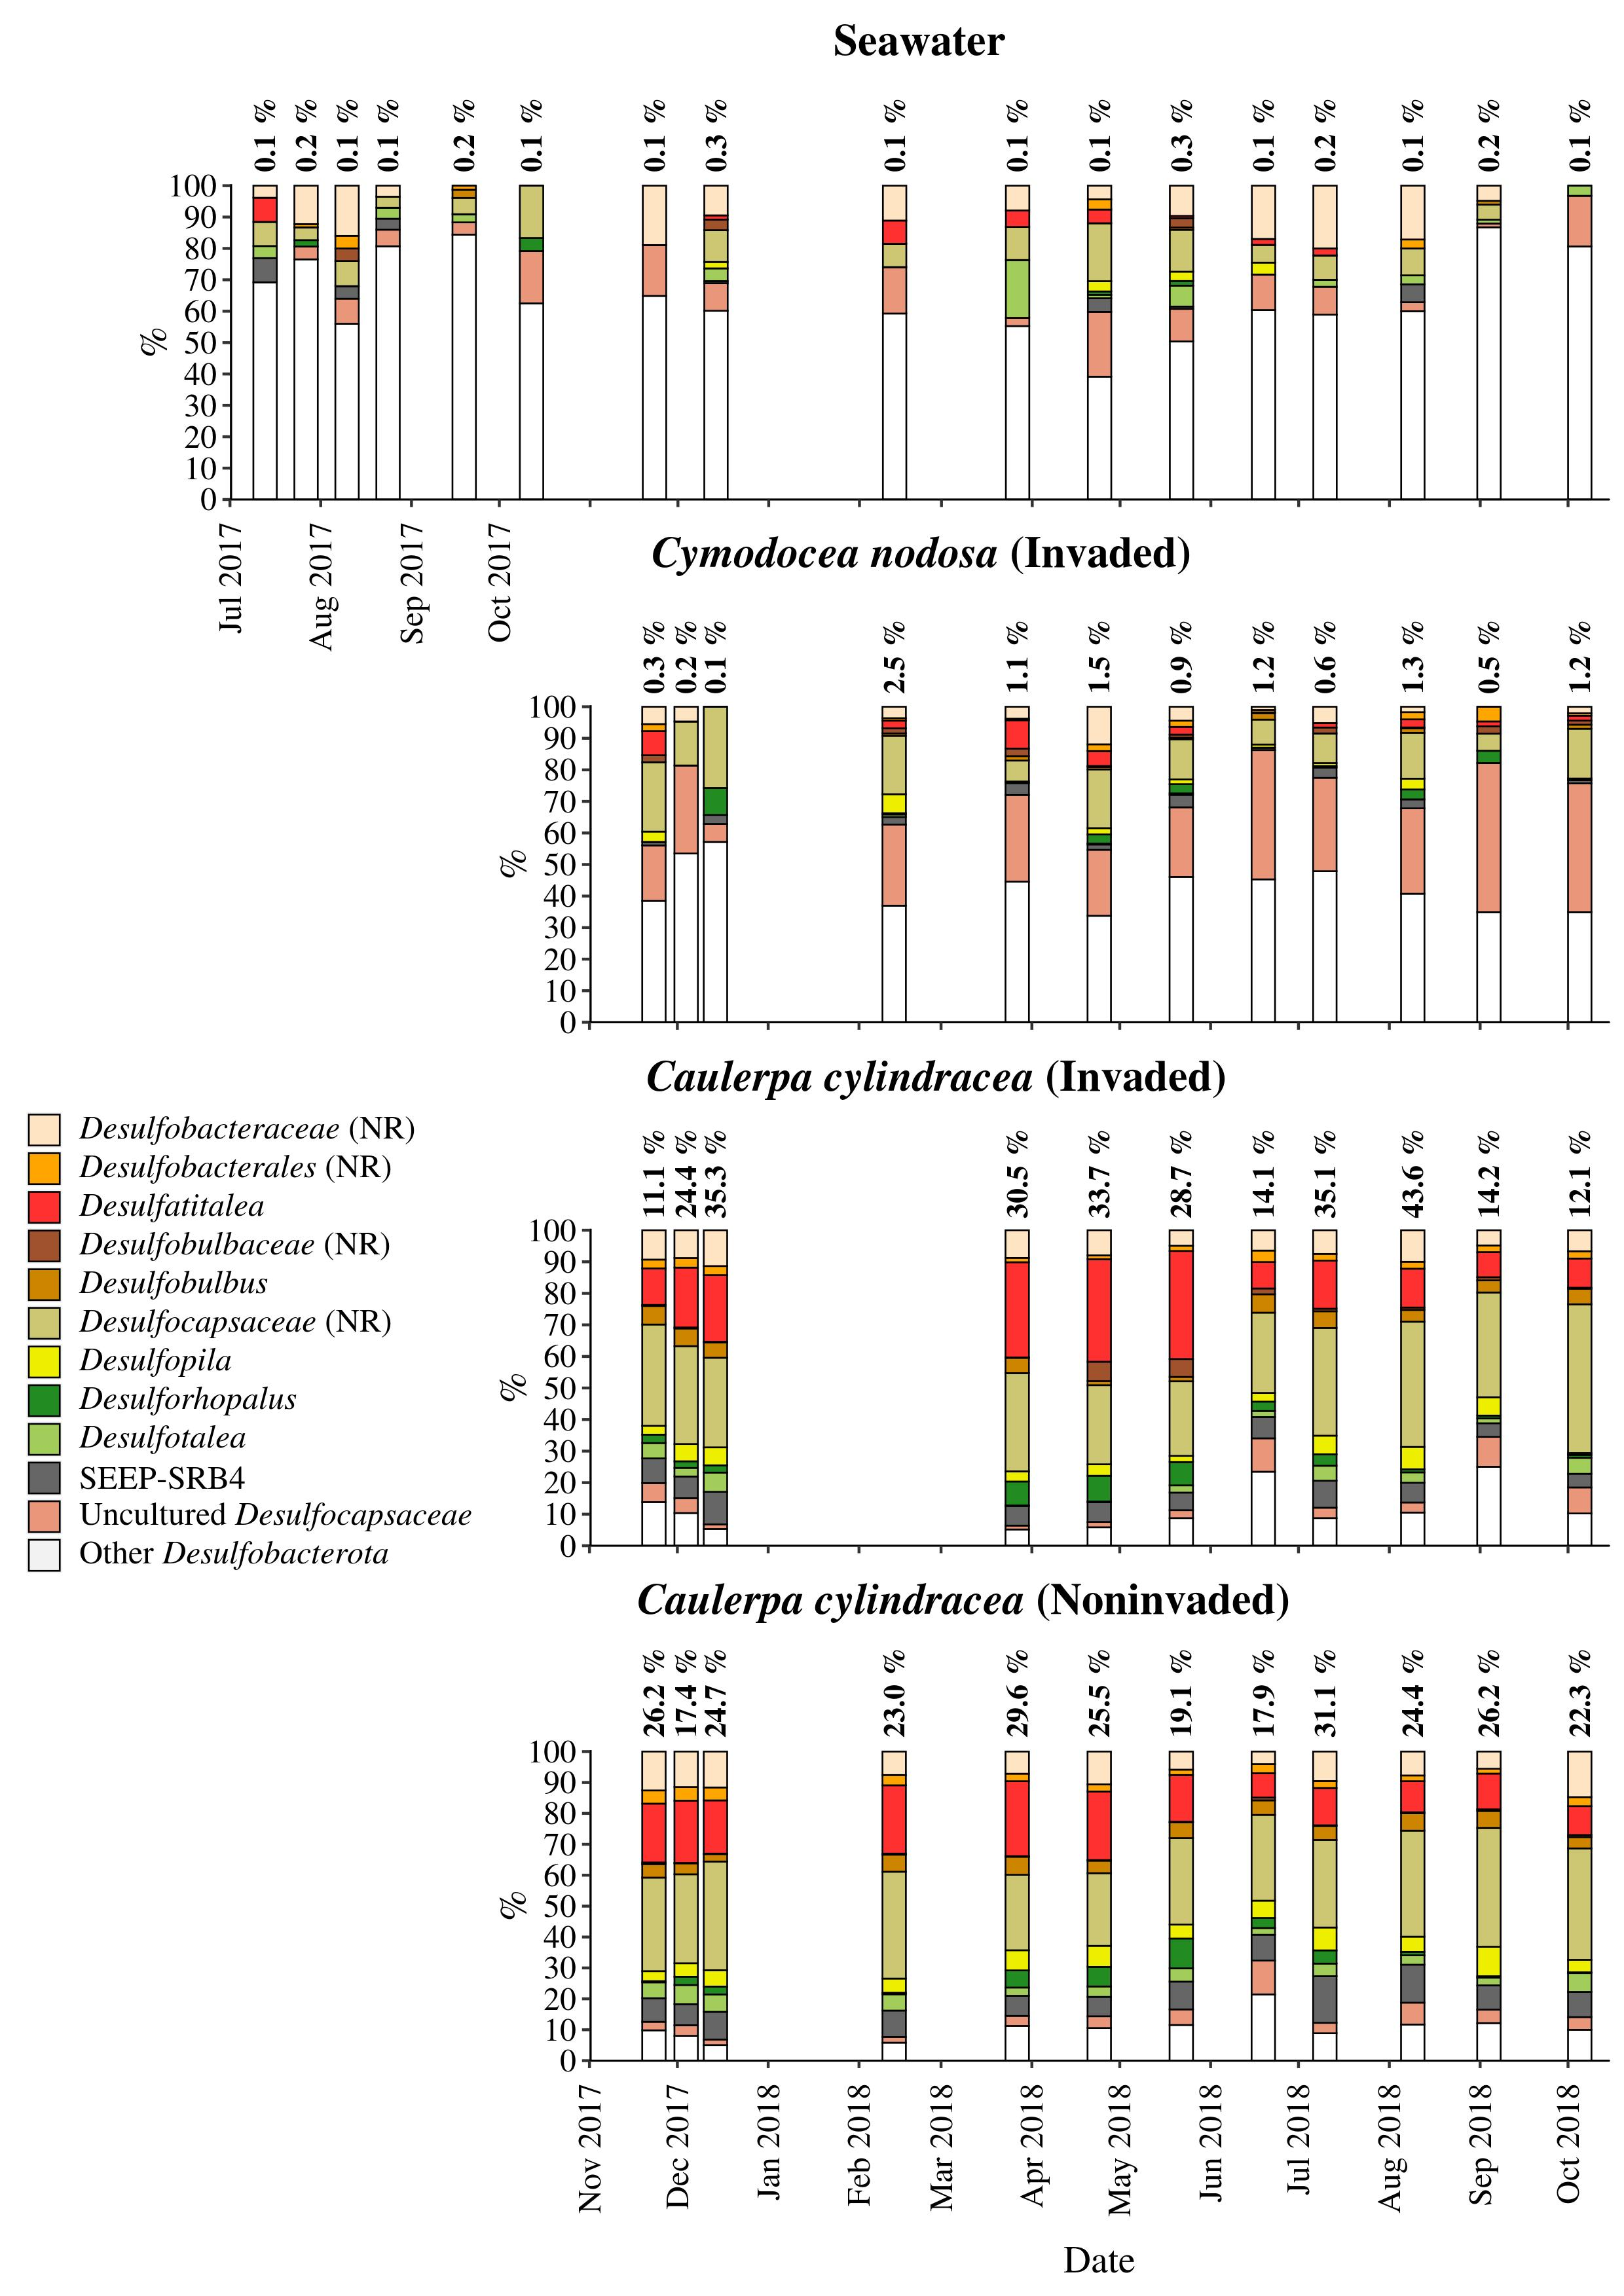
\includegraphics[width=0.85\linewidth]{../results/figures/desulfobacterota_bar_plot} 

}

\caption{Taxonomic classification and relative contribution of the most abundant (> 1 \si{\percent}) sequences within the \textit{Desulfobacterota} on the surfaces of the macrophytes \textit{C. nodosa} (mixed settlement) and \textit{C. cylindracea} (mixed and monospecific settlement) and in the ambient seawater. The proportion of sequences classified as \textit{Desulfobacterota} in the total bacterial and archaeal community is given above the corresponding bar. NR -- No Relative (sequences without known relatives within the corresponding group)\label{desulfo}}\label{fig:unnamed-chunk-9}
\end{figure}


\end{document}
